% Auto-generated by generate_ltt_appendix_tex.py — do not edit by hand (change generate_ltt_appendix_tex.py and re-run ``python generate_ltt_appendix_tex.py``).

\subsection*{Class 1 (II)}
\noindent Representative of this ep-isomorphism class.\\
\noindent Distinguished indices:\\ $\{1, 8, 11, 19, 53, 60, 63, 65, 71, 80, 103, 110, 124, 125, 154, 160, 164, 165, 241, 244, 251, 257, 261, 268\}$, $24$ total.
\begin{center}
\resizebox{\linewidth}{!}{%
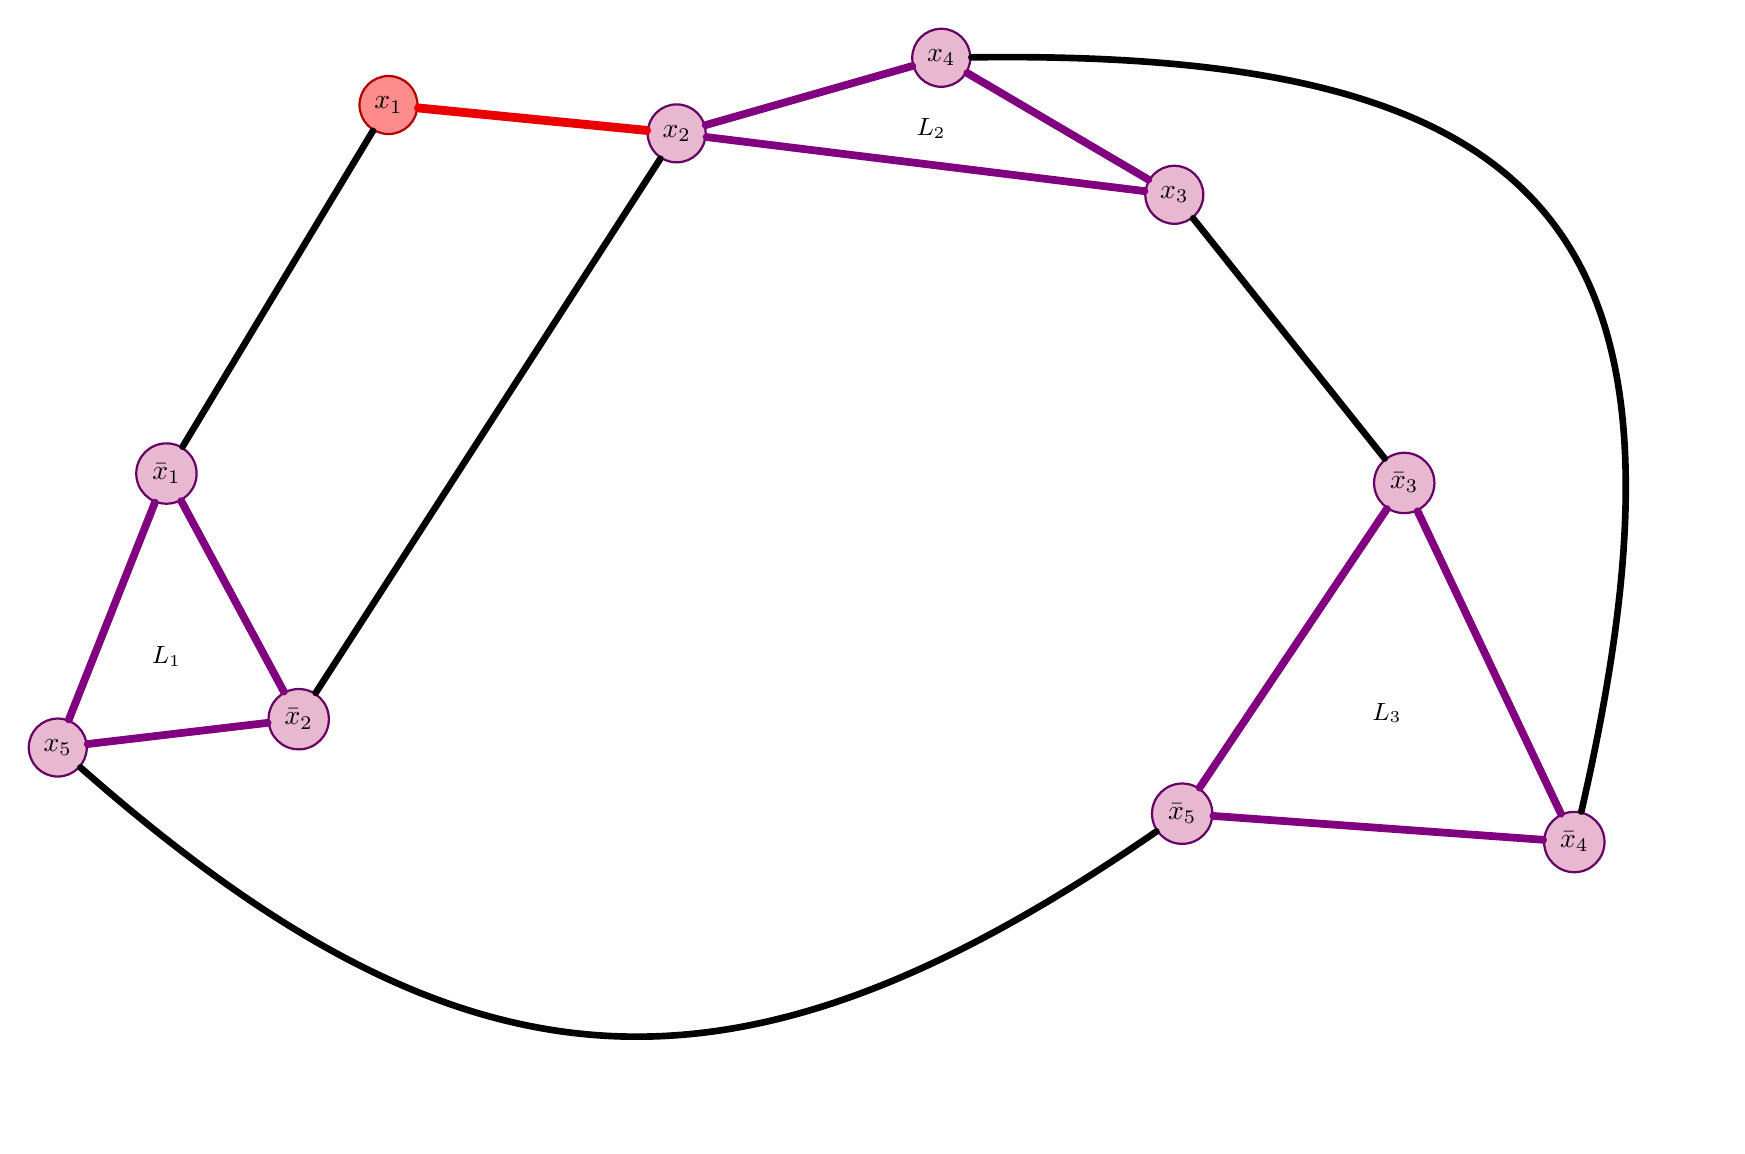
\begin{tikzpicture}[
  lbl/.style={font=\small, inner sep=1pt},
  redv/.style={circle, draw=red!70!black, line width=0.8pt, fill=red!45, minimum size=7mm},
  purpv/.style={circle, draw=violet!80!black, line width=0.8pt, fill=blue!12!purple!28, minimum size=7mm},
  purpleedge/.style={draw=violet, line width=2.8pt, line cap=round, line join=round},
  blackedge/.style={draw=black, line width=2.4pt, line cap=round},
  rededge/.style={draw=red!92!black, line width=3.2pt, line cap=round}
]

\node[redv] (nx1) at (-3.84, 6.54) {$x_{1}$};
\node[purpv] (nb1) at (-6.66, 1.86) {$\bar{x}_{1}$};
\node[purpv] (nx2) at (-0.18, 6.18) {$x_{2}$};
\node[purpv] (nb2) at (-4.98, -1.26) {$\bar{x}_{2}$};
\node[purpv] (nx3) at (6.14, 5.40) {$x_{3}$};
\node[purpv] (nb3) at (9.06, 1.74) {$\bar{x}_{3}$};
\node[purpv] (nx4) at (3.18, 7.14) {$x_{4}$};
\node[purpv] (nb4) at (11.22, -2.82) {$\bar{x}_{4}$};
\node[purpv] (nx5) at (-8.04, -1.62) {$x_{5}$};
\node[purpv] (nb5) at (6.24, -2.46) {$\bar{x}_{5}$};
\draw[purpleedge] (nb1) -- (nb2);
\draw[purpleedge] (nb1) -- (nx5);
\draw[purpleedge] (nb2) -- (nx5);
\draw[purpleedge] (nx2) -- (nx3);
\draw[purpleedge] (nx2) -- (nx4);
\draw[purpleedge] (nx3) -- (nx4);
\draw[purpleedge] (nb3) -- (nb4);
\draw[purpleedge] (nb3) -- (nb5);
\draw[purpleedge] (nb4) -- (nb5);
\draw[blackedge] (nx1) -- (nb1);
\draw[blackedge] (nx2) -- (nb2);
\draw[blackedge] (nx3) -- (nb3);
\draw[blackedge] (nx4) .. controls (11.06,7.25) and (12.99,4.86) .. (nb4);
\draw[blackedge] (nx5) .. controls (-2.86,-6.18) and (0.56,-6.38) .. (nb5);
\draw[rededge] (nx1) -- (nx2);
\node[lbl] at (-6.66, -0.46) {$L_1$};
\node[lbl] at (3.05, 6.24) {$L_2$};
\node[lbl] at (8.84, -1.18) {$L_3$};

\end{tikzpicture}%
}%

\end{center}
\medskip
\subsection*{Class 2 (I)}
\noindent Representative of this ep-isomorphism class.\\
\noindent Distinguished indices:\\ $\{2, 3, 5, 6, 12, 14, 15, 17, 51, 52, 57, 59, 61, 62, 66, 68, 73, 74, 76, 77, 101, 102, 107, 109\\ 121, 122, 127, 129, 151, 152, 156, 158, 161, 162, 167, 169, 245, 246, 249, 250, 252, 253, 259, 260, 262, 263, 265, 266\}$, $48$ total.
\begin{center}
\resizebox{\linewidth}{!}{%
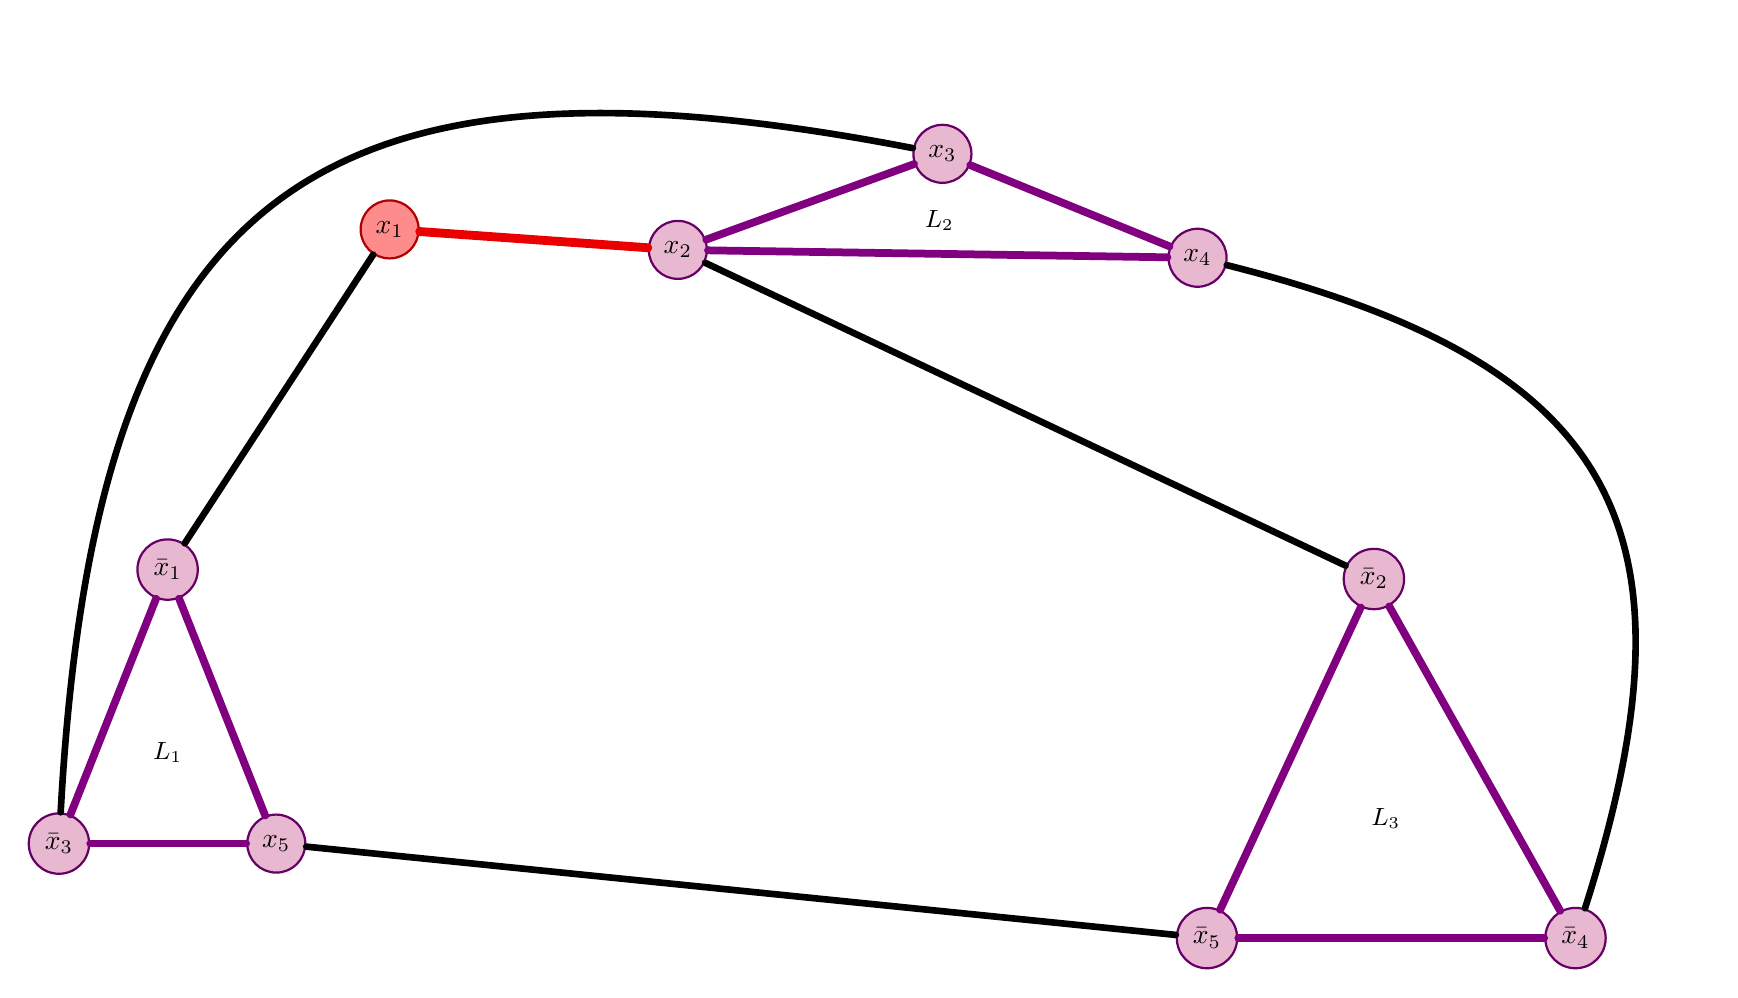
\begin{tikzpicture}[
  lbl/.style={font=\small, inner sep=1pt},
  redv/.style={circle, draw=red!70!black, line width=0.8pt, fill=red!45, minimum size=7mm},
  purpv/.style={circle, draw=violet!80!black, line width=0.8pt, fill=blue!12!purple!28, minimum size=7mm},
  purpleedge/.style={draw=violet, line width=2.8pt, line cap=round, line join=round},
  blackedge/.style={draw=black, line width=2.4pt, line cap=round},
  rededge/.style={draw=red!92!black, line width=3.2pt, line cap=round}
]

\node[redv] (nx1) at (-3.84, 6.18) {$x_{1}$};
\node[purpv] (nb1) at (-6.66, 1.86) {$\bar{x}_{1}$};
\node[purpv] (nx2) at (-0.18, 5.92) {$x_{2}$};
\node[purpv] (nb2) at (8.66, 1.74) {$\bar{x}_{2}$};
\node[purpv] (nx3) at (3.18, 7.14) {$x_{3}$};
\node[purpv] (nb3) at (-8.04, -1.62) {$\bar{x}_{3}$};
\node[purpv] (nx4) at (6.42, 5.82) {$x_{4}$};
\node[purpv] (nb4) at (11.22, -2.82) {$\bar{x}_{4}$};
\node[purpv] (nx5) at (-5.28, -1.62) {$x_{5}$};
\node[purpv] (nb5) at (6.54, -2.82) {$\bar{x}_{5}$};
\draw[purpleedge] (nb1) -- (nb3);
\draw[purpleedge] (nb1) -- (nx5);
\draw[purpleedge] (nb3) -- (nx5);
\draw[purpleedge] (nx2) -- (nx3);
\draw[purpleedge] (nx2) -- (nx4);
\draw[purpleedge] (nx3) -- (nx4);
\draw[purpleedge] (nb2) -- (nb4);
\draw[purpleedge] (nb2) -- (nb5);
\draw[purpleedge] (nb4) -- (nb5);
\draw[blackedge] (nx1) -- (nb1);
\draw[blackedge] (nx2) -- (nb2);
\draw[blackedge] (nx3) .. controls (-4.90,8.70) and (-7.59,6.60) .. (nb3);
\draw[blackedge] (nx4) .. controls (11.74,4.48) and (12.89,2.41) .. (nb4);
\draw[blackedge] (nx5) -- (nb5);
\draw[rededge] (nx1) -- (nx2);
\node[lbl] at (-6.66, -0.46) {$L_1$};
\node[lbl] at (3.14, 6.29) {$L_2$};
\node[lbl] at (8.81, -1.30) {$L_3$};

\end{tikzpicture}%
}%

\end{center}
\medskip
\subsection*{Class 3 (VII)}
\noindent Representative of this ep-isomorphism class.\\
\noindent Distinguished indices: $\{4, 13, 58, 67, 72, 108, 126, 159, 166, 243, 256, 269\}$, $12$ total.
\begin{center}
\resizebox{\linewidth}{!}{%
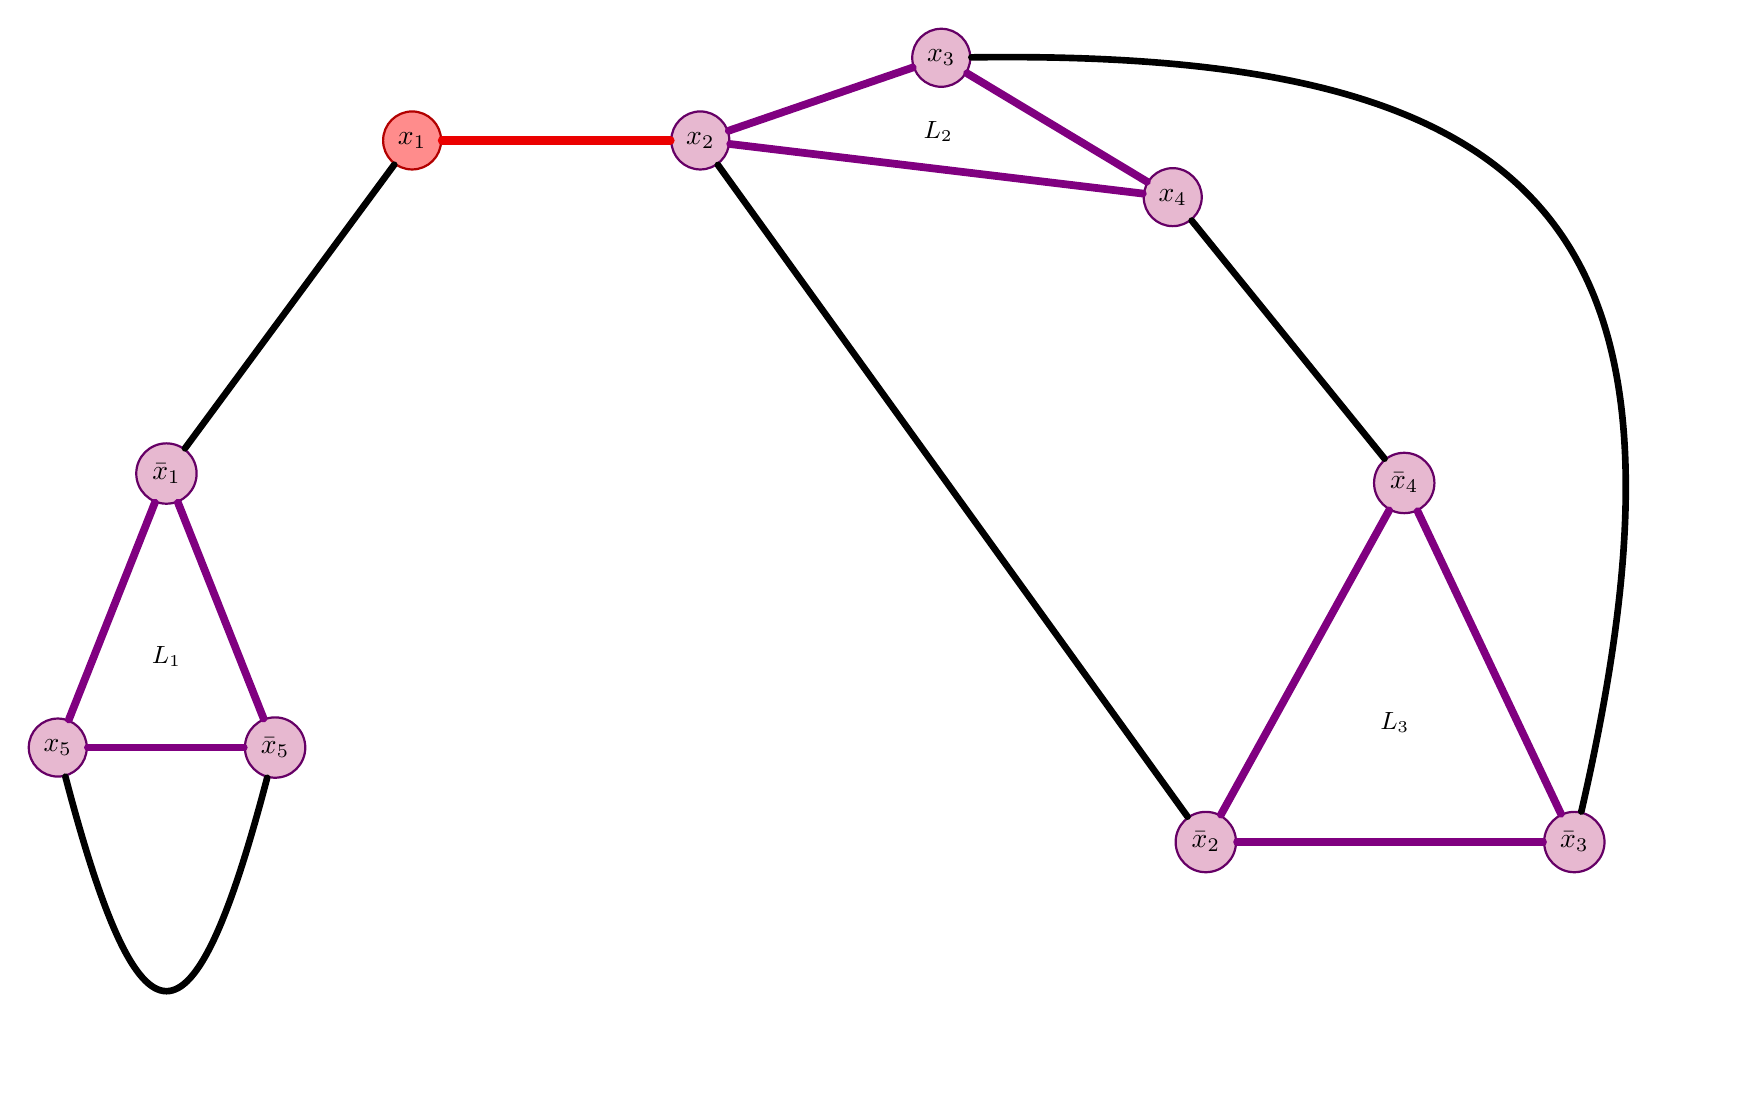
\begin{tikzpicture}[
  lbl/.style={font=\small, inner sep=1pt},
  redv/.style={circle, draw=red!70!black, line width=0.8pt, fill=red!45, minimum size=7mm},
  purpv/.style={circle, draw=violet!80!black, line width=0.8pt, fill=blue!12!purple!28, minimum size=7mm},
  purpleedge/.style={draw=violet, line width=2.8pt, line cap=round, line join=round},
  blackedge/.style={draw=black, line width=2.4pt, line cap=round},
  rededge/.style={draw=red!92!black, line width=3.2pt, line cap=round}
]

\node[redv] (nx1) at (-3.54, 6.09) {$x_{1}$};
\node[purpv] (nb1) at (-6.66, 1.86) {$\bar{x}_{1}$};
\node[purpv] (nx2) at (0.12, 6.09) {$x_{2}$};
\node[purpv] (nb2) at (6.54, -2.82) {$\bar{x}_{2}$};
\node[purpv] (nx3) at (3.18, 7.14) {$x_{3}$};
\node[purpv] (nb3) at (11.22, -2.82) {$\bar{x}_{3}$};
\node[purpv] (nx4) at (6.12, 5.37) {$x_{4}$};
\node[purpv] (nb4) at (9.06, 1.74) {$\bar{x}_{4}$};
\node[purpv] (nx5) at (-8.04, -1.62) {$x_{5}$};
\node[purpv] (nb5) at (-5.28, -1.62) {$\bar{x}_{5}$};
\draw[purpleedge] (nb1) -- (nx5);
\draw[purpleedge] (nb1) -- (nb5);
\draw[purpleedge] (nx5) -- (nb5);
\draw[purpleedge] (nx2) -- (nx3);
\draw[purpleedge] (nx2) -- (nx4);
\draw[purpleedge] (nx3) -- (nx4);
\draw[purpleedge] (nb2) -- (nb3);
\draw[purpleedge] (nb2) -- (nb4);
\draw[purpleedge] (nb3) -- (nb4);
\draw[blackedge] (nx1) -- (nb1);
\draw[blackedge] (nx2) -- (nb2);
\draw[blackedge] (nx3) .. controls (11.06,7.25) and (12.99,4.86) .. (nb3);
\draw[blackedge] (nx4) -- (nb4);
\draw[blackedge] (nx5) .. controls (-6.99,-5.62) and (-6.33,-5.62) .. (nb5);
\draw[rededge] (nx1) -- (nx2);
\node[lbl] at (-6.66, -0.46) {$L_1$};
\node[lbl] at (3.14, 6.20) {$L_2$};
\node[lbl] at (8.94, -1.30) {$L_3$};

\end{tikzpicture}%
}%

\end{center}
\medskip
\subsection*{Class 4 (VIII)}
\noindent Representative of this ep-isomorphism class.\\
\noindent Distinguished indices: $\{7, 16, 56, 69, 75, 106, 128, 157, 168, 242, 255, 270\}$, $12$ total.
\begin{center}
\resizebox{\linewidth}{!}{%
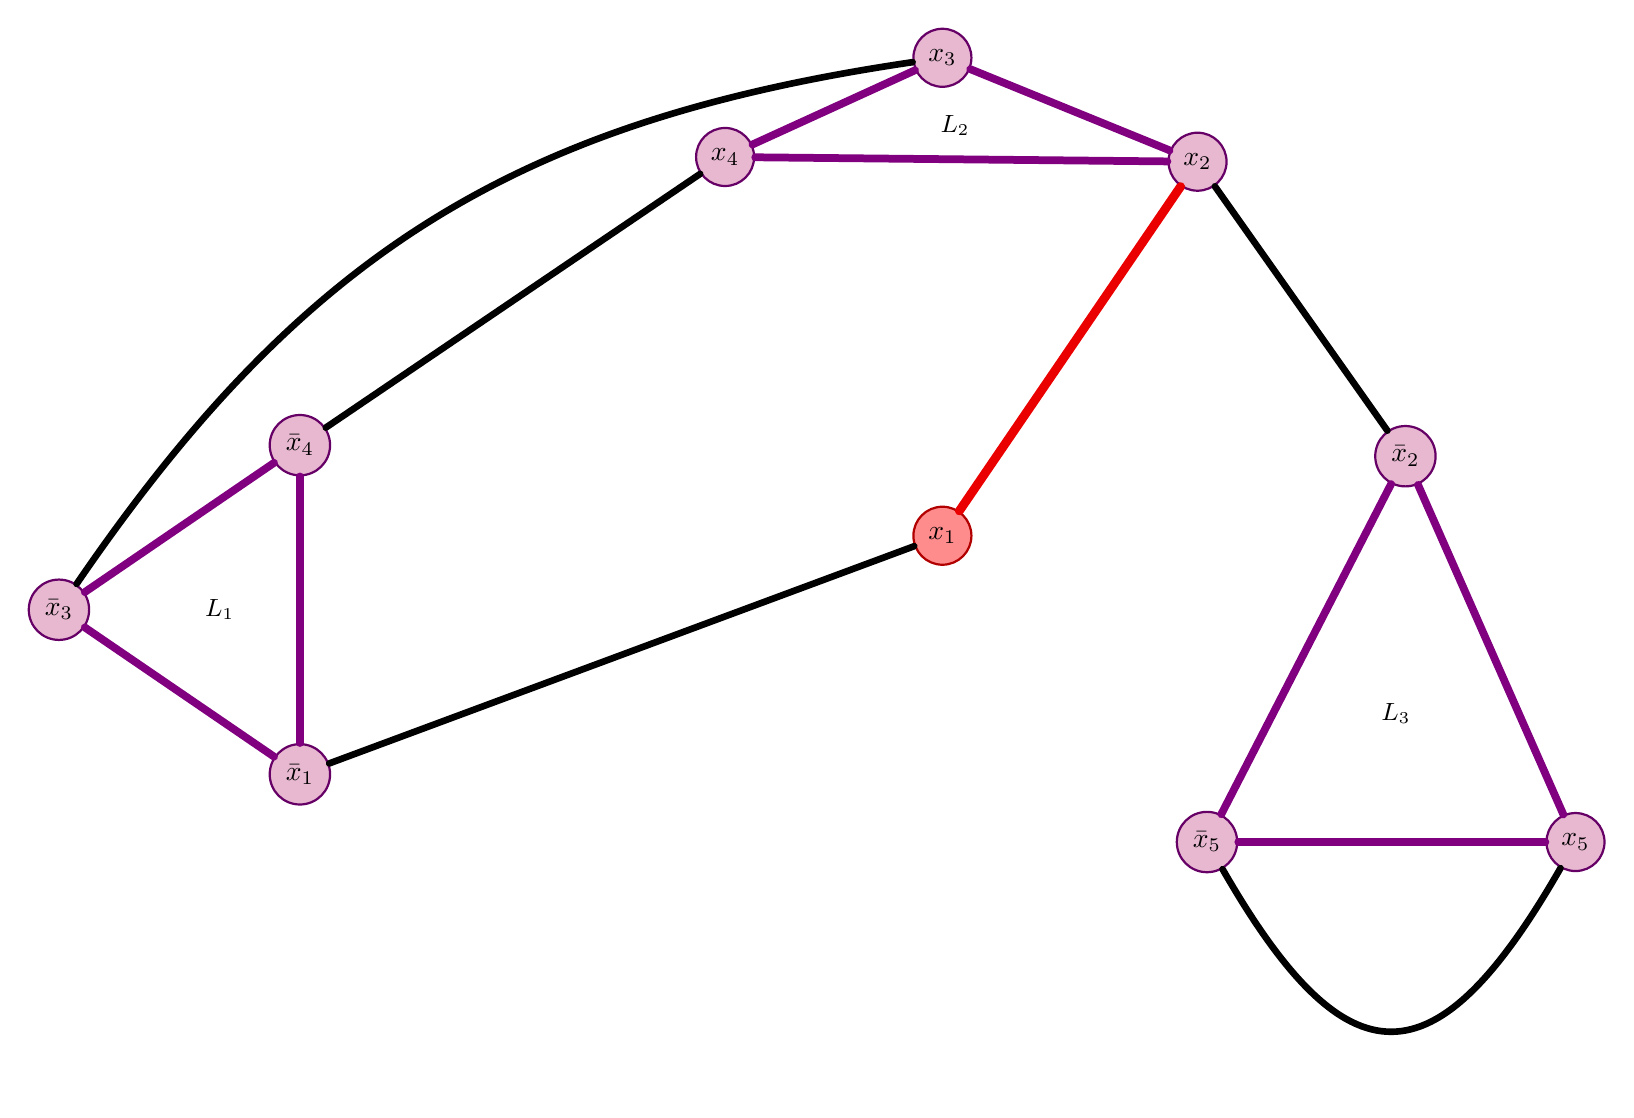
\begin{tikzpicture}[
  lbl/.style={font=\small, inner sep=1pt},
  redv/.style={circle, draw=red!70!black, line width=0.8pt, fill=red!45, minimum size=7mm},
  purpv/.style={circle, draw=violet!80!black, line width=0.8pt, fill=blue!12!purple!28, minimum size=7mm},
  purpleedge/.style={draw=violet, line width=2.8pt, line cap=round, line join=round},
  blackedge/.style={draw=black, line width=2.4pt, line cap=round},
  rededge/.style={draw=red!92!black, line width=3.2pt, line cap=round}
]

\node[redv] (nx1) at (3.18, 1.07) {$x_{1}$};
\node[purpv] (nb1) at (-4.98, -1.96) {$\bar{x}_{1}$};
\node[purpv] (nx2) at (6.42, 5.82) {$x_{2}$};
\node[purpv] (nb2) at (9.06, 2.08) {$\bar{x}_{2}$};
\node[purpv] (nx3) at (3.18, 7.14) {$x_{3}$};
\node[purpv] (nb3) at (-8.04, 0.13) {$\bar{x}_{3}$};
\node[purpv] (nx4) at (0.42, 5.88) {$x_{4}$};
\node[purpv] (nb4) at (-4.98, 2.22) {$\bar{x}_{4}$};
\node[purpv] (nx5) at (11.22, -2.82) {$x_{5}$};
\node[purpv] (nb5) at (6.54, -2.82) {$\bar{x}_{5}$};
\draw[purpleedge] (nb1) -- (nb3);
\draw[purpleedge] (nb1) -- (nb4);
\draw[purpleedge] (nb3) -- (nb4);
\draw[purpleedge] (nx2) -- (nx3);
\draw[purpleedge] (nx2) -- (nx4);
\draw[purpleedge] (nx3) -- (nx4);
\draw[purpleedge] (nb2) -- (nx5);
\draw[purpleedge] (nb2) -- (nb5);
\draw[purpleedge] (nx5) -- (nb5);
\draw[blackedge] (nx1) -- (nb1);
\draw[blackedge] (nx2) -- (nb2);
\draw[blackedge] (nx3) .. controls (-2.25,6.34) and (-4.94,4.66) .. (nb3);
\draw[blackedge] (nx4) -- (nb4);
\draw[blackedge] (nx5) .. controls (9.44,-5.92) and (8.32,-5.92) .. (nb5);
\draw[rededge] (nx1) -- (nx2);
\node[lbl] at (-6.00, 0.13) {$L_1$};
\node[lbl] at (3.34, 6.28) {$L_2$};
\node[lbl] at (8.94, -1.19) {$L_3$};

\end{tikzpicture}%
}%

\end{center}
\medskip
\subsection*{Class 5 (VI)}
\noindent Representative of this ep-isomorphism class.\\
\noindent Distinguished indices:\\ $\{9, 10, 18, 20, 54, 55, 64, 70, 78, 79, 104, 105, 123, 130, 153, 155, 163, 170, 247, 248, 254, 258, 264, 267\}$, $24$ total.
\begin{center}
\resizebox{\linewidth}{!}{%
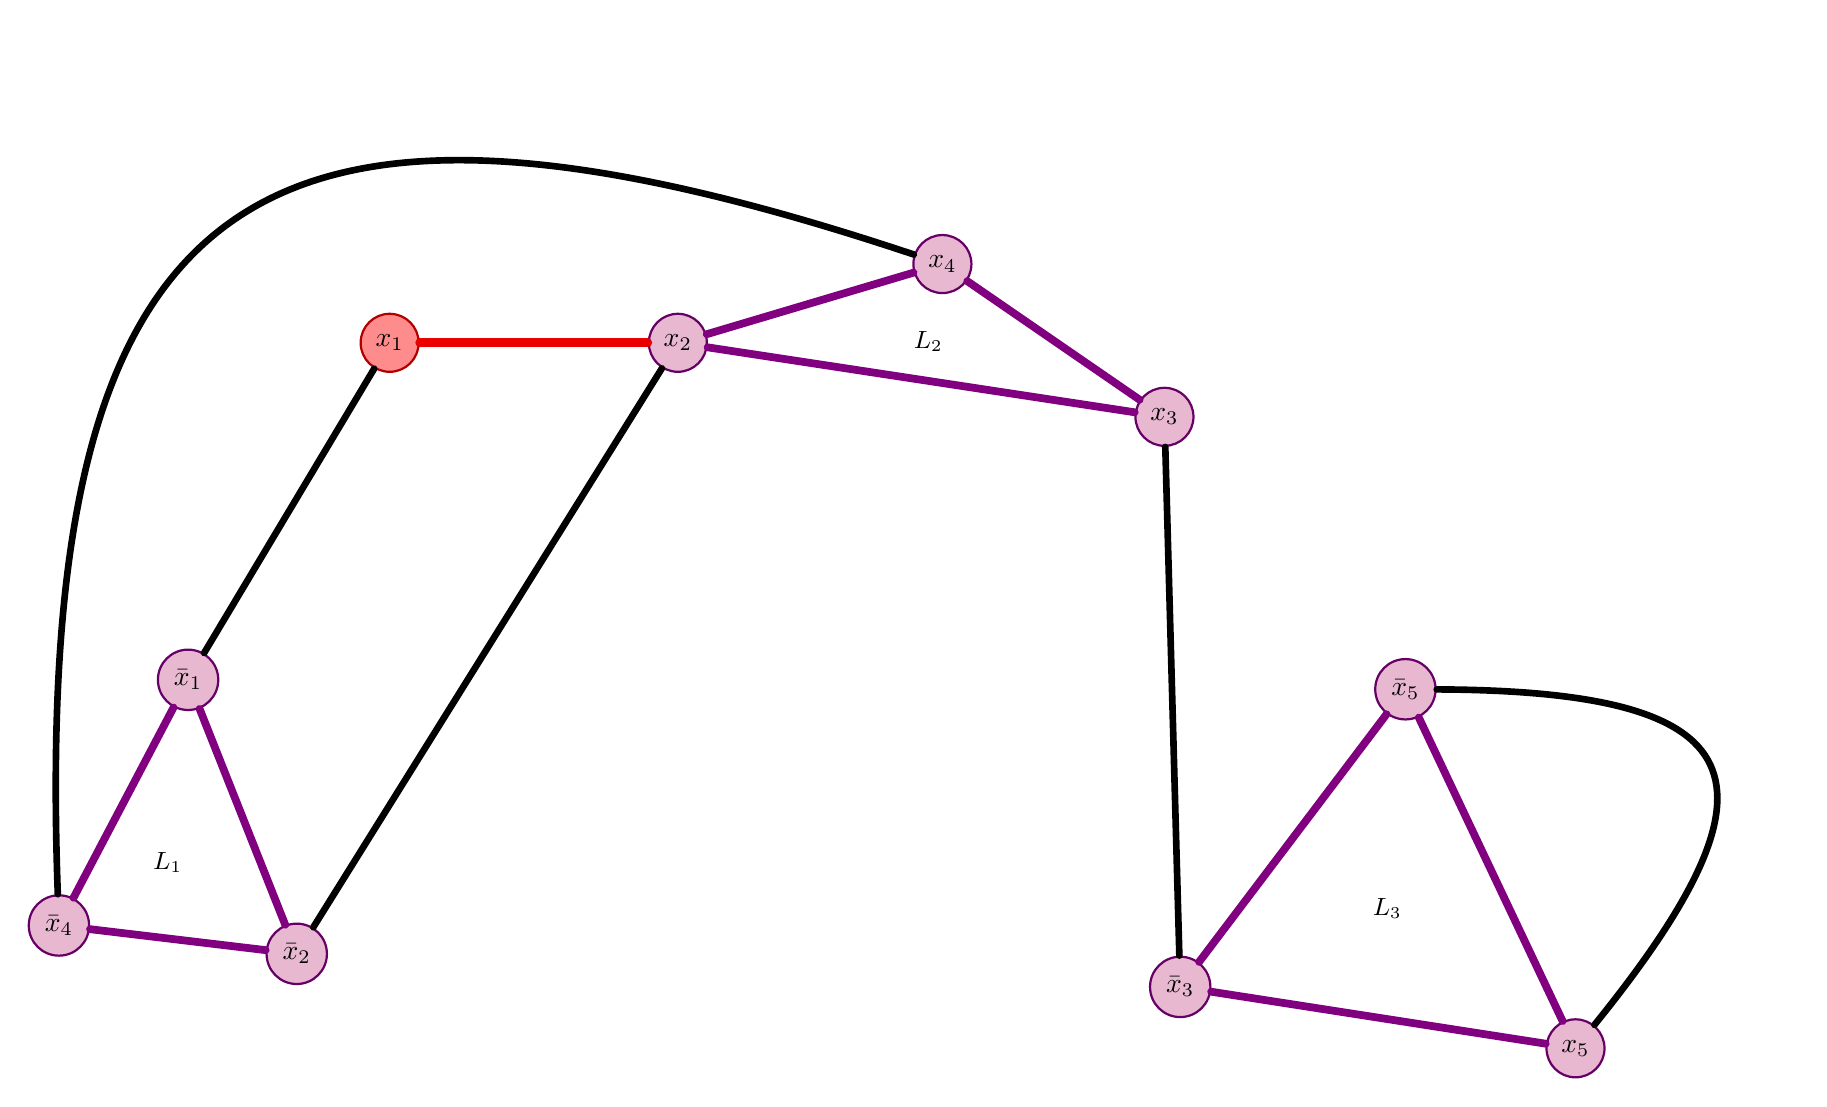
\begin{tikzpicture}[
  lbl/.style={font=\small, inner sep=1pt},
  redv/.style={circle, draw=red!70!black, line width=0.8pt, fill=red!45, minimum size=7mm},
  purpv/.style={circle, draw=violet!80!black, line width=0.8pt, fill=blue!12!purple!28, minimum size=7mm},
  purpleedge/.style={draw=violet, line width=2.8pt, line cap=round, line join=round},
  blackedge/.style={draw=black, line width=2.4pt, line cap=round},
  rededge/.style={draw=red!92!black, line width=3.2pt, line cap=round}
]

\node[redv] (nx1) at (-3.84, 6.14) {$x_{1}$};
\node[purpv] (nb1) at (-6.40, 1.86) {$\bar{x}_{1}$};
\node[purpv] (nx2) at (-0.18, 6.14) {$x_{2}$};
\node[purpv] (nb2) at (-5.02, -1.62) {$\bar{x}_{2}$};
\node[purpv] (nx3) at (6.00, 5.20) {$x_{3}$};
\node[purpv] (nb3) at (6.20, -2.04) {$\bar{x}_{3}$};
\node[purpv] (nx4) at (3.18, 7.14) {$x_{4}$};
\node[purpv] (nb4) at (-8.04, -1.26) {$\bar{x}_{4}$};
\node[purpv] (nx5) at (11.22, -2.82) {$x_{5}$};
\node[purpv] (nb5) at (9.06, 1.74) {$\bar{x}_{5}$};
\draw[purpleedge] (nb1) -- (nb2);
\draw[purpleedge] (nb1) -- (nb4);
\draw[purpleedge] (nb2) -- (nb4);
\draw[purpleedge] (nx2) -- (nx3);
\draw[purpleedge] (nx2) -- (nx4);
\draw[purpleedge] (nx3) -- (nx4);
\draw[purpleedge] (nb3) -- (nx5);
\draw[purpleedge] (nb3) -- (nb5);
\draw[purpleedge] (nx5) -- (nb5);
\draw[blackedge] (nx1) -- (nb1);
\draw[blackedge] (nx2) -- (nb2);
\draw[blackedge] (nx3) -- (nb3);
\draw[blackedge] (nx4) .. controls (-5.69,10.10) and (-8.38,8.09) .. (nb4);
\draw[blackedge] (nx5) .. controls (14.01,0.63) and (13.50,1.72) .. (nb5);
\draw[rededge] (nx1) -- (nx2);
\node[lbl] at (-6.66, -0.46) {$L_1$};
\node[lbl] at (3.00, 6.16) {$L_2$};
\node[lbl] at (8.83, -1.04) {$L_3$};

\end{tikzpicture}%
}%

\end{center}
\medskip
\subsection*{Class 6 (III)}
\noindent Representative of this ep-isomorphism class.\\
\noindent Distinguished indices:\\ $\{21, 22, 27, 29, 81, 83, 87, 90, 131, 134, 136, 140, 181, 184, 186, 190, 191, 194, 195, 199, 201, 202, 207, 209\}$, $24$ total.
\begin{center}
\resizebox{\linewidth}{!}{%
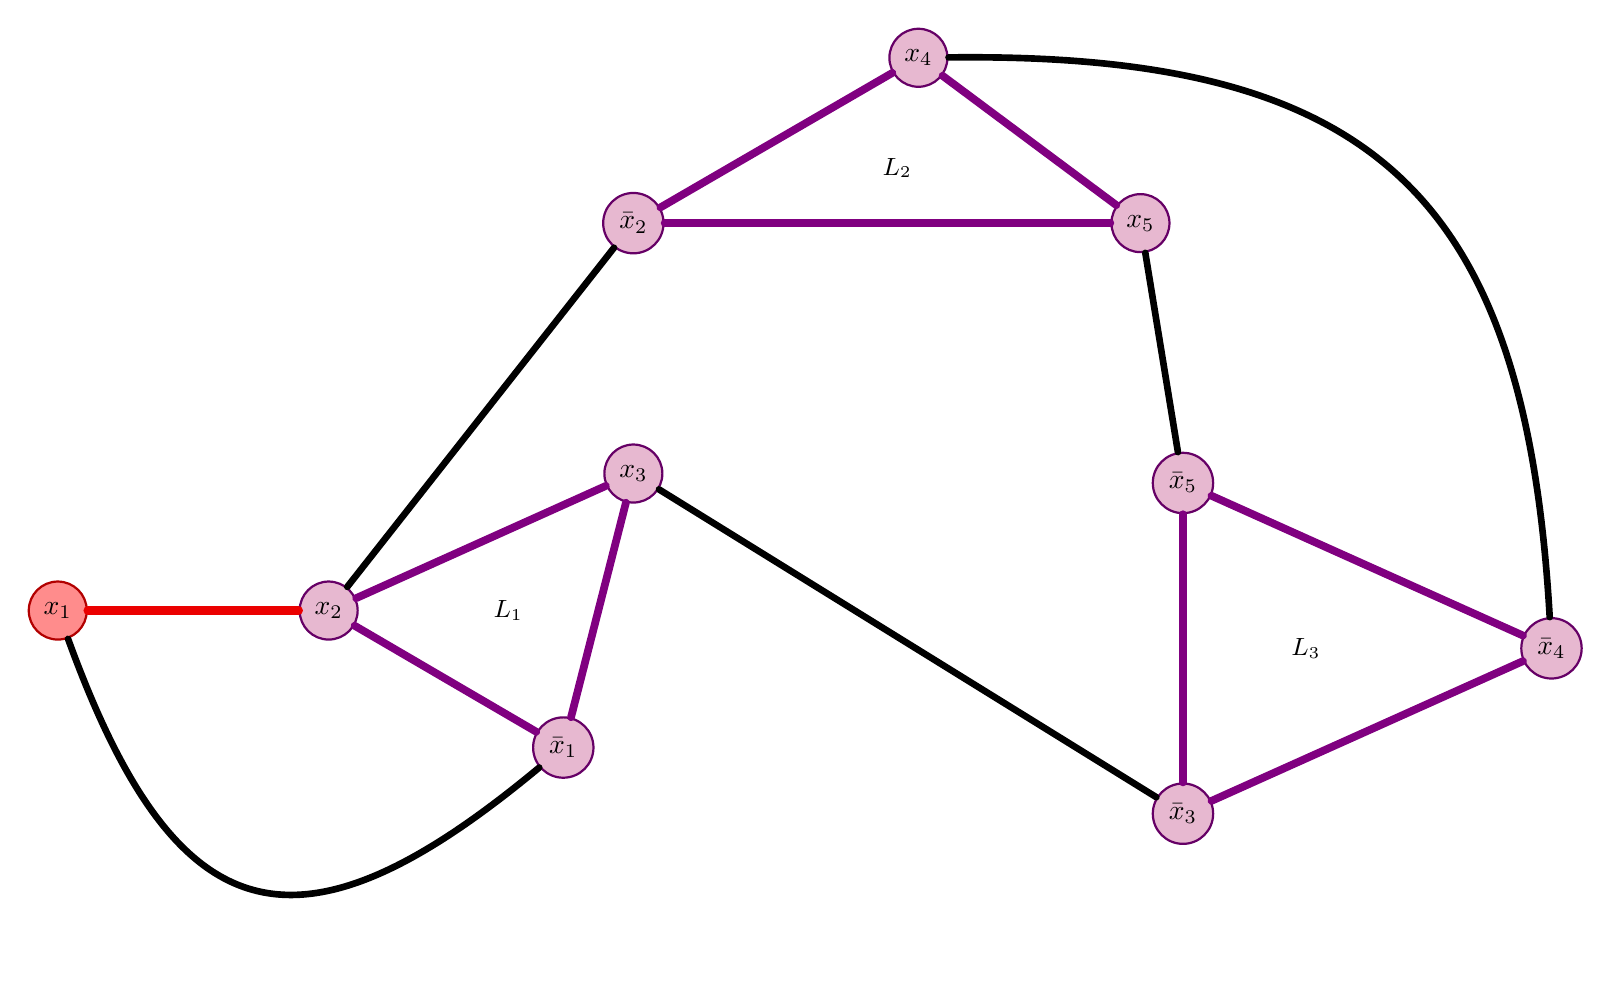
\begin{tikzpicture}[
  lbl/.style={font=\small, inner sep=1pt},
  redv/.style={circle, draw=red!70!black, line width=0.8pt, fill=red!45, minimum size=7mm},
  purpv/.style={circle, draw=violet!80!black, line width=0.8pt, fill=blue!12!purple!28, minimum size=7mm},
  purpleedge/.style={draw=violet, line width=2.8pt, line cap=round, line join=round},
  blackedge/.style={draw=black, line width=2.4pt, line cap=round},
  rededge/.style={draw=red!92!black, line width=3.2pt, line cap=round}
]

\node[redv] (nx1) at (-7.75, 0.12) {$x_{1}$};
\node[purpv] (nb1) at (-1.33, -1.62) {$\bar{x}_{1}$};
\node[purpv] (nx2) at (-4.31, 0.12) {$x_{2}$};
\node[purpv] (nb2) at (-0.44, 5.04) {$\bar{x}_{2}$};
\node[purpv] (nx3) at (-0.44, 1.86) {$x_{3}$};
\node[purpv] (nb3) at (6.54, -2.46) {$\bar{x}_{3}$};
\node[purpv] (nx4) at (3.18, 7.14) {$x_{4}$};
\node[purpv] (nb4) at (11.22, -0.36) {$\bar{x}_{4}$};
\node[purpv] (nx5) at (6.00, 5.04) {$x_{5}$};
\node[purpv] (nb5) at (6.54, 1.74) {$\bar{x}_{5}$};
\draw[purpleedge] (nb1) -- (nx2);
\draw[purpleedge] (nb1) -- (nx3);
\draw[purpleedge] (nx2) -- (nx3);
\draw[purpleedge] (nb2) -- (nx4);
\draw[purpleedge] (nb2) -- (nx5);
\draw[purpleedge] (nx4) -- (nx5);
\draw[purpleedge] (nb3) -- (nb4);
\draw[purpleedge] (nb3) -- (nb5);
\draw[purpleedge] (nb4) -- (nb5);
\draw[blackedge] (nx1) .. controls (-6.25,-4.01) and (-4.71,-4.43) .. (nb1);
\draw[blackedge] (nx2) -- (nb2);
\draw[blackedge] (nx3) -- (nb3);
\draw[blackedge] (nx4) .. controls (8.96,7.21) and (10.89,5.41) .. (nb4);
\draw[blackedge] (nx5) -- (nb5);
\draw[rededge] (nx1) -- (nx2);
\node[lbl] at (-2.03, 0.12) {$L_1$};
\node[lbl] at (2.91, 5.74) {$L_2$};
\node[lbl] at (8.10, -0.36) {$L_3$};

\end{tikzpicture}%
}%

\end{center}
\medskip
\subsection*{Class 7 (X)}
\noindent Representative of this ep-isomorphism class.\\
\noindent Distinguished indices:\\ $\{23, 24, 25, 30, 82, 84, 86, 89, 132, 133, 137, 138, 182, 185, 188, 189, 192, 196, 197, 200, 203, 204, 205, 210\}$, $24$ total.
\begin{center}
\resizebox{\linewidth}{!}{%
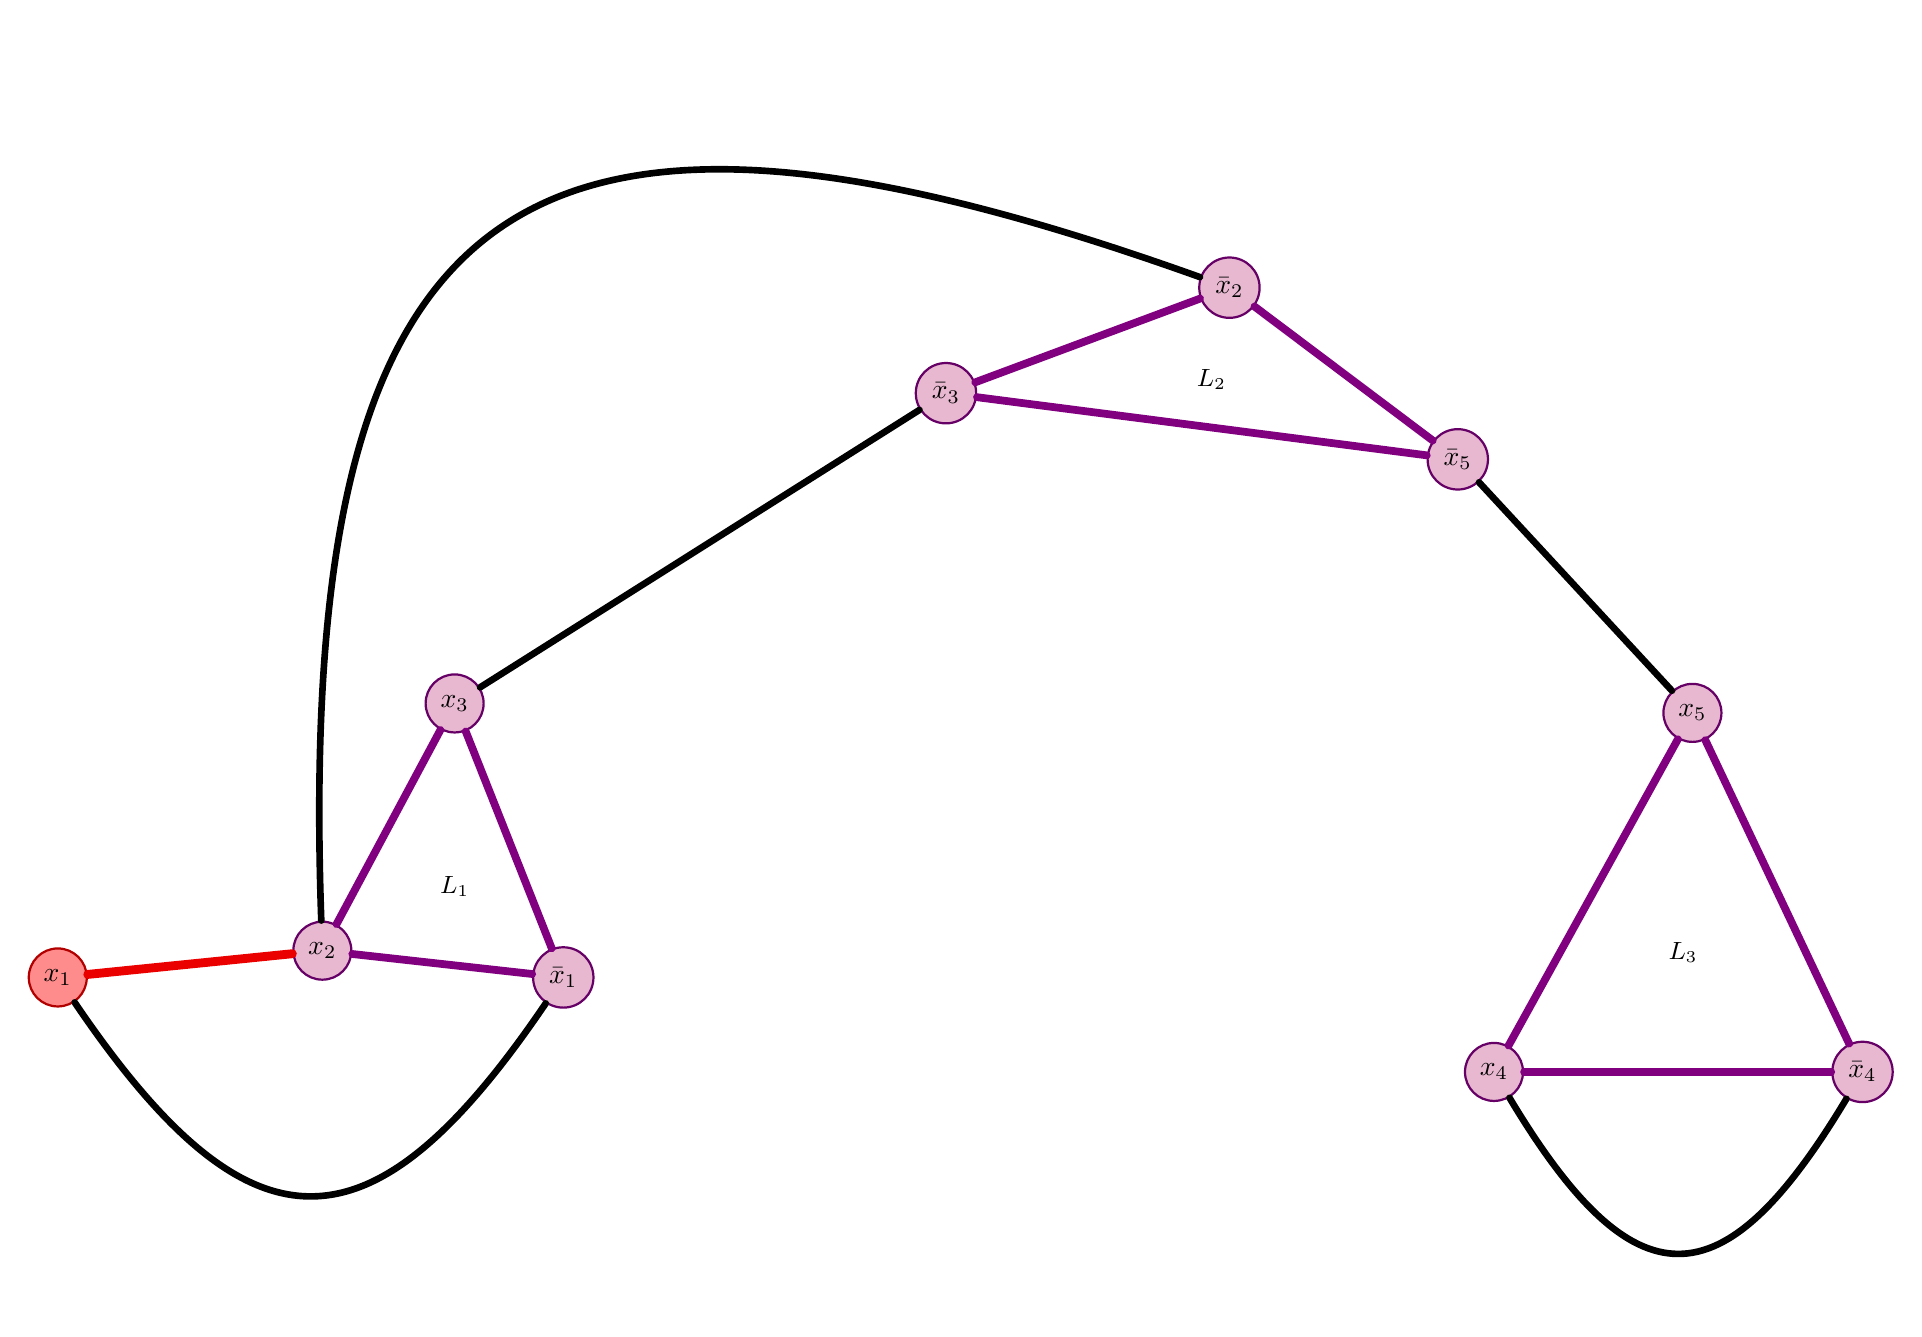
\begin{tikzpicture}[
  lbl/.style={font=\small, inner sep=1pt},
  redv/.style={circle, draw=red!70!black, line width=0.8pt, fill=red!45, minimum size=7mm},
  purpv/.style={circle, draw=violet!80!black, line width=0.8pt, fill=blue!12!purple!28, minimum size=7mm},
  purpleedge/.style={draw=violet, line width=2.8pt, line cap=round, line join=round},
  blackedge/.style={draw=black, line width=2.4pt, line cap=round},
  rededge/.style={draw=red!92!black, line width=3.2pt, line cap=round}
]

\node[redv] (nx1) at (-11.70, -1.62) {$x_{1}$};
\node[purpv] (nb1) at (-5.28, -1.62) {$\bar{x}_{1}$};
\node[purpv] (nx2) at (-8.34, -1.28) {$x_{2}$};
\node[purpv] (nb2) at (3.18, 7.14) {$\bar{x}_{2}$};
\node[purpv] (nx3) at (-6.66, 1.86) {$x_{3}$};
\node[purpv] (nb3) at (-0.42, 5.80) {$\bar{x}_{3}$};
\node[purpv] (nx4) at (6.54, -2.82) {$x_{4}$};
\node[purpv] (nb4) at (11.22, -2.82) {$\bar{x}_{4}$};
\node[purpv] (nx5) at (9.06, 1.74) {$x_{5}$};
\node[purpv] (nb5) at (6.08, 4.96) {$\bar{x}_{5}$};
\draw[purpleedge] (nb1) -- (nx2);
\draw[purpleedge] (nb1) -- (nx3);
\draw[purpleedge] (nx2) -- (nx3);
\draw[purpleedge] (nb2) -- (nb3);
\draw[purpleedge] (nb2) -- (nb5);
\draw[purpleedge] (nb3) -- (nb5);
\draw[purpleedge] (nx4) -- (nb4);
\draw[purpleedge] (nx4) -- (nx5);
\draw[purpleedge] (nb4) -- (nx5);
\draw[blackedge] (nx1) .. controls (-9.26,-5.22) and (-7.72,-5.22) .. (nb1);
\draw[blackedge] (nx2) .. controls (-8.68,8.38) and (-5.92,10.40) .. (nb2);
\draw[blackedge] (nx3) -- (nb3);
\draw[blackedge] (nx4) .. controls (8.32,-5.79) and (9.44,-5.79) .. (nb4);
\draw[blackedge] (nx5) -- (nb5);
\draw[rededge] (nx1) -- (nx2);
\node[lbl] at (-6.66, -0.46) {$L_1$};
\node[lbl] at (2.95, 5.97) {$L_2$};
\node[lbl] at (8.94, -1.30) {$L_3$};

\end{tikzpicture}%
}%

\end{center}
\medskip
\subsection*{Class 8 (XII)}
\noindent Representative of this ep-isomorphism class.\\
\noindent Distinguished indices: $\{26, 28, 85, 88, 135, 139, 183, 187, 193, 198, 206, 208\}$, $12$ total.
\begin{center}
\resizebox{\linewidth}{!}{%
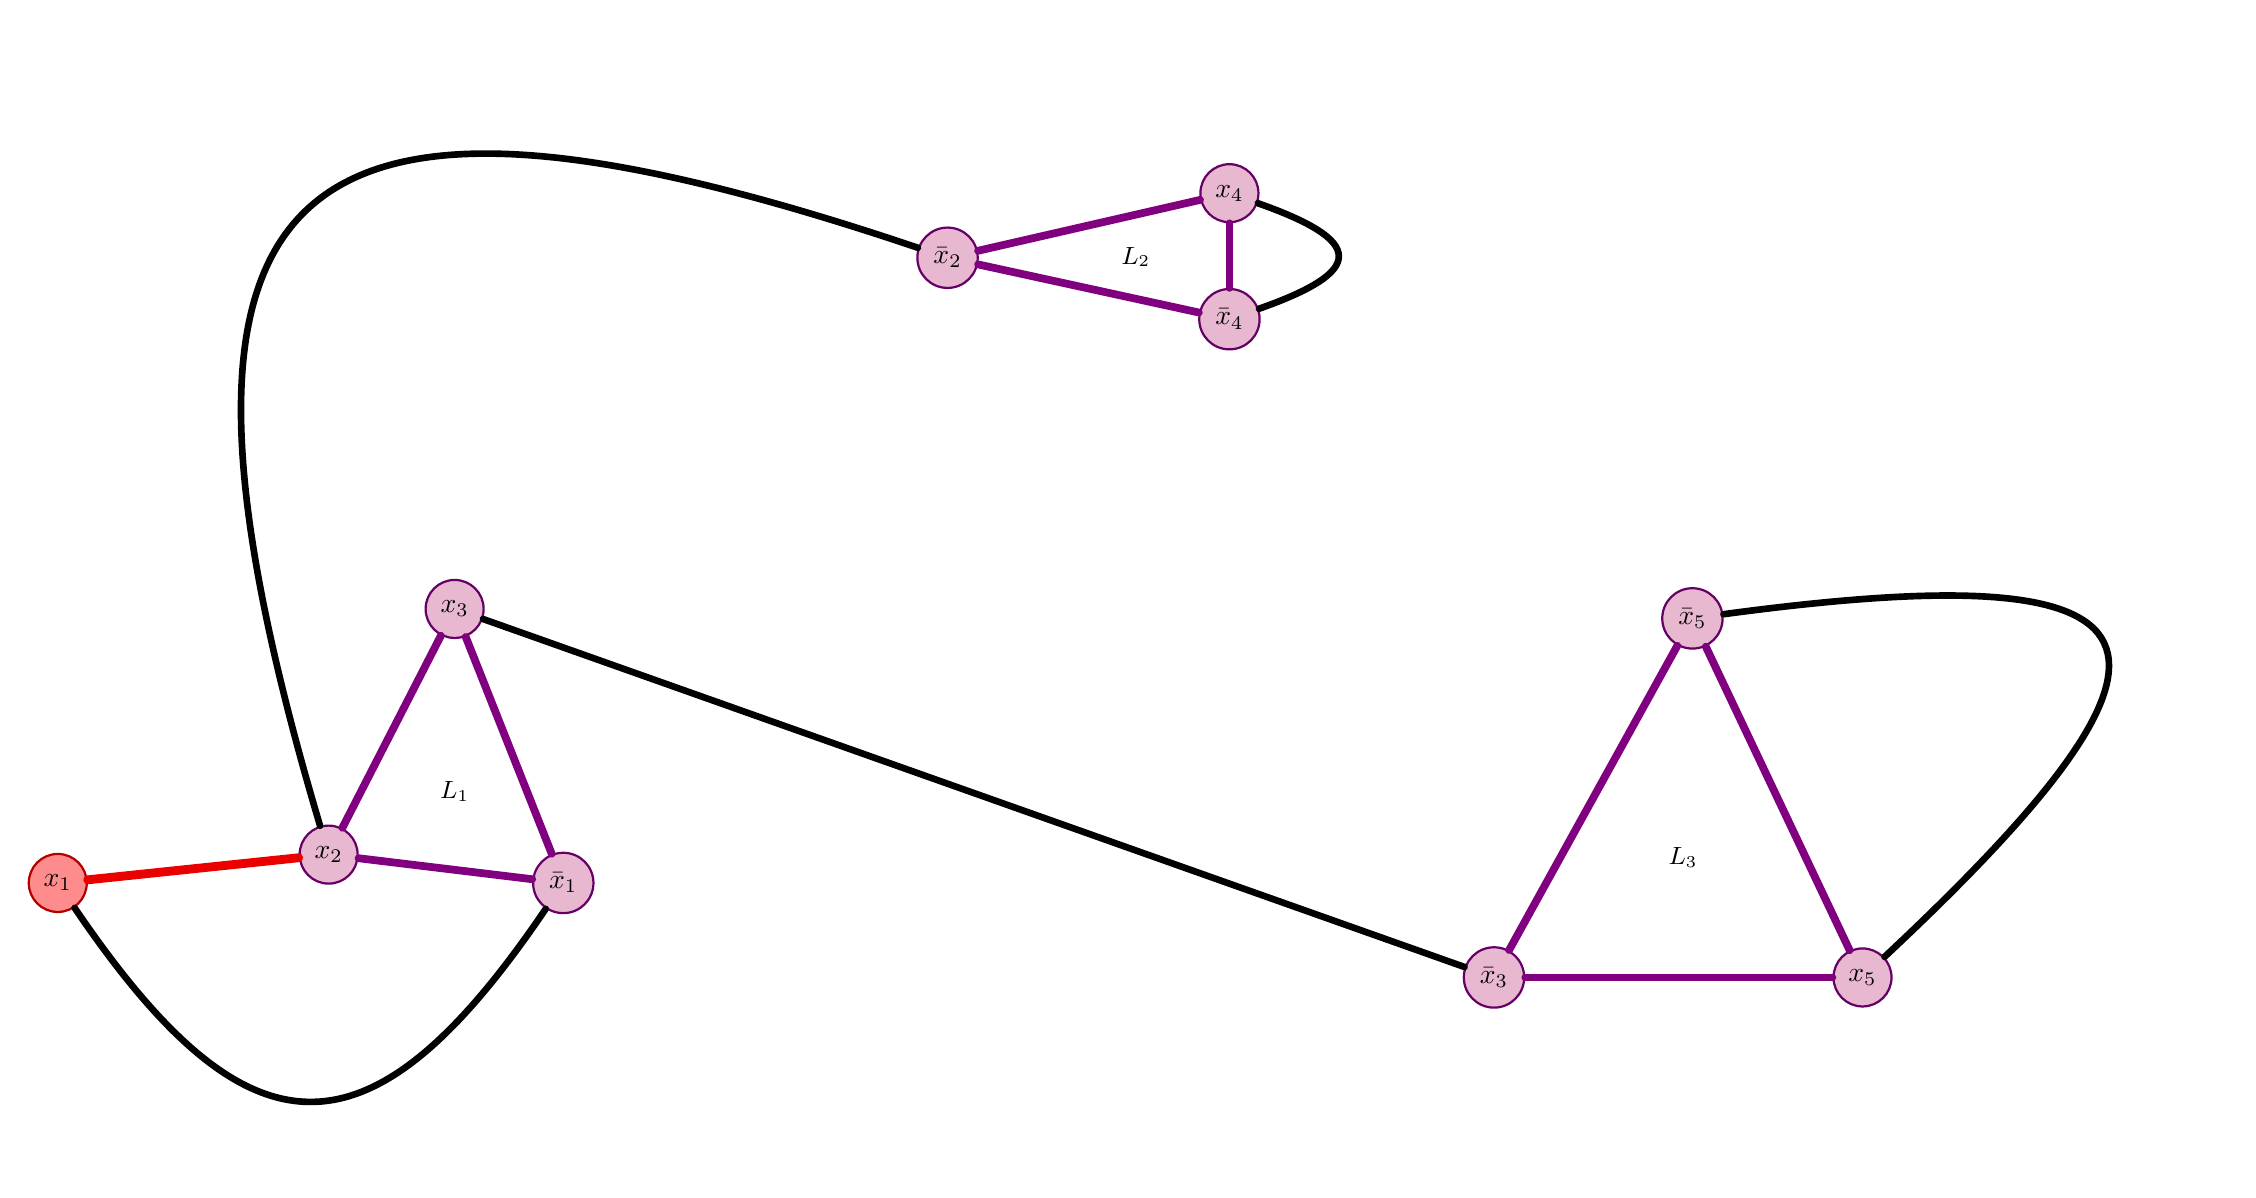
\begin{tikzpicture}[
  lbl/.style={font=\small, inner sep=1pt},
  redv/.style={circle, draw=red!70!black, line width=0.8pt, fill=red!45, minimum size=7mm},
  purpv/.style={circle, draw=violet!80!black, line width=0.8pt, fill=blue!12!purple!28, minimum size=7mm},
  purpleedge/.style={draw=violet, line width=2.8pt, line cap=round, line join=round},
  blackedge/.style={draw=black, line width=2.4pt, line cap=round},
  rededge/.style={draw=red!92!black, line width=3.2pt, line cap=round}
]

\node[redv] (nx1) at (-11.70, -1.62) {$x_{1}$};
\node[purpv] (nb1) at (-5.28, -1.62) {$\bar{x}_{1}$};
\node[purpv] (nx2) at (-8.26, -1.26) {$x_{2}$};
\node[purpv] (nb2) at (-0.40, 6.32) {$\bar{x}_{2}$};
\node[purpv] (nx3) at (-6.66, 1.86) {$x_{3}$};
\node[purpv] (nb3) at (6.54, -2.82) {$\bar{x}_{3}$};
\node[purpv] (nx4) at (3.18, 7.14) {$x_{4}$};
\node[purpv] (nb4) at (3.18, 5.54) {$\bar{x}_{4}$};
\node[purpv] (nx5) at (11.22, -2.82) {$x_{5}$};
\node[purpv] (nb5) at (9.06, 1.74) {$\bar{x}_{5}$};
\draw[purpleedge] (nb1) -- (nx2);
\draw[purpleedge] (nb1) -- (nx3);
\draw[purpleedge] (nx2) -- (nx3);
\draw[purpleedge] (nb2) -- (nx4);
\draw[purpleedge] (nb2) -- (nb4);
\draw[purpleedge] (nx4) -- (nb4);
\draw[purpleedge] (nb3) -- (nx5);
\draw[purpleedge] (nb3) -- (nb5);
\draw[purpleedge] (nx5) -- (nb5);
\draw[blackedge] (nx1) .. controls (-9.26,-5.22) and (-7.72,-5.22) .. (nb1);
\draw[blackedge] (nx2) .. controls (-10.83,7.38) and (-8.94,9.20) .. (nb2);
\draw[blackedge] (nx3) -- (nb3);
\draw[blackedge] (nx4) .. controls (4.91,6.53) and (4.91,6.15) .. (nb4);
\draw[blackedge] (nx5) .. controls (15.82,1.48) and (15.30,2.58) .. (nb5);
\draw[rededge] (nx1) -- (nx2);
\node[lbl] at (-6.66, -0.46) {$L_1$};
\node[lbl] at (1.99, 6.33) {$L_2$};
\node[lbl] at (8.94, -1.30) {$L_3$};

\end{tikzpicture}%
}%

\end{center}
\medskip
\subsection*{Class 9 (IV)}
\noindent Representative of this ep-isomorphism class.\\
\noindent Distinguished indices:\\ $\{31, 32, 37, 39, 91, 93, 97, 100, 141, 144, 146, 150, 211, 214, 216, 220, 221, 224, 225, 229, 231, 232, 237, 239\}$, $24$ total.
\begin{center}
\resizebox{\linewidth}{!}{%
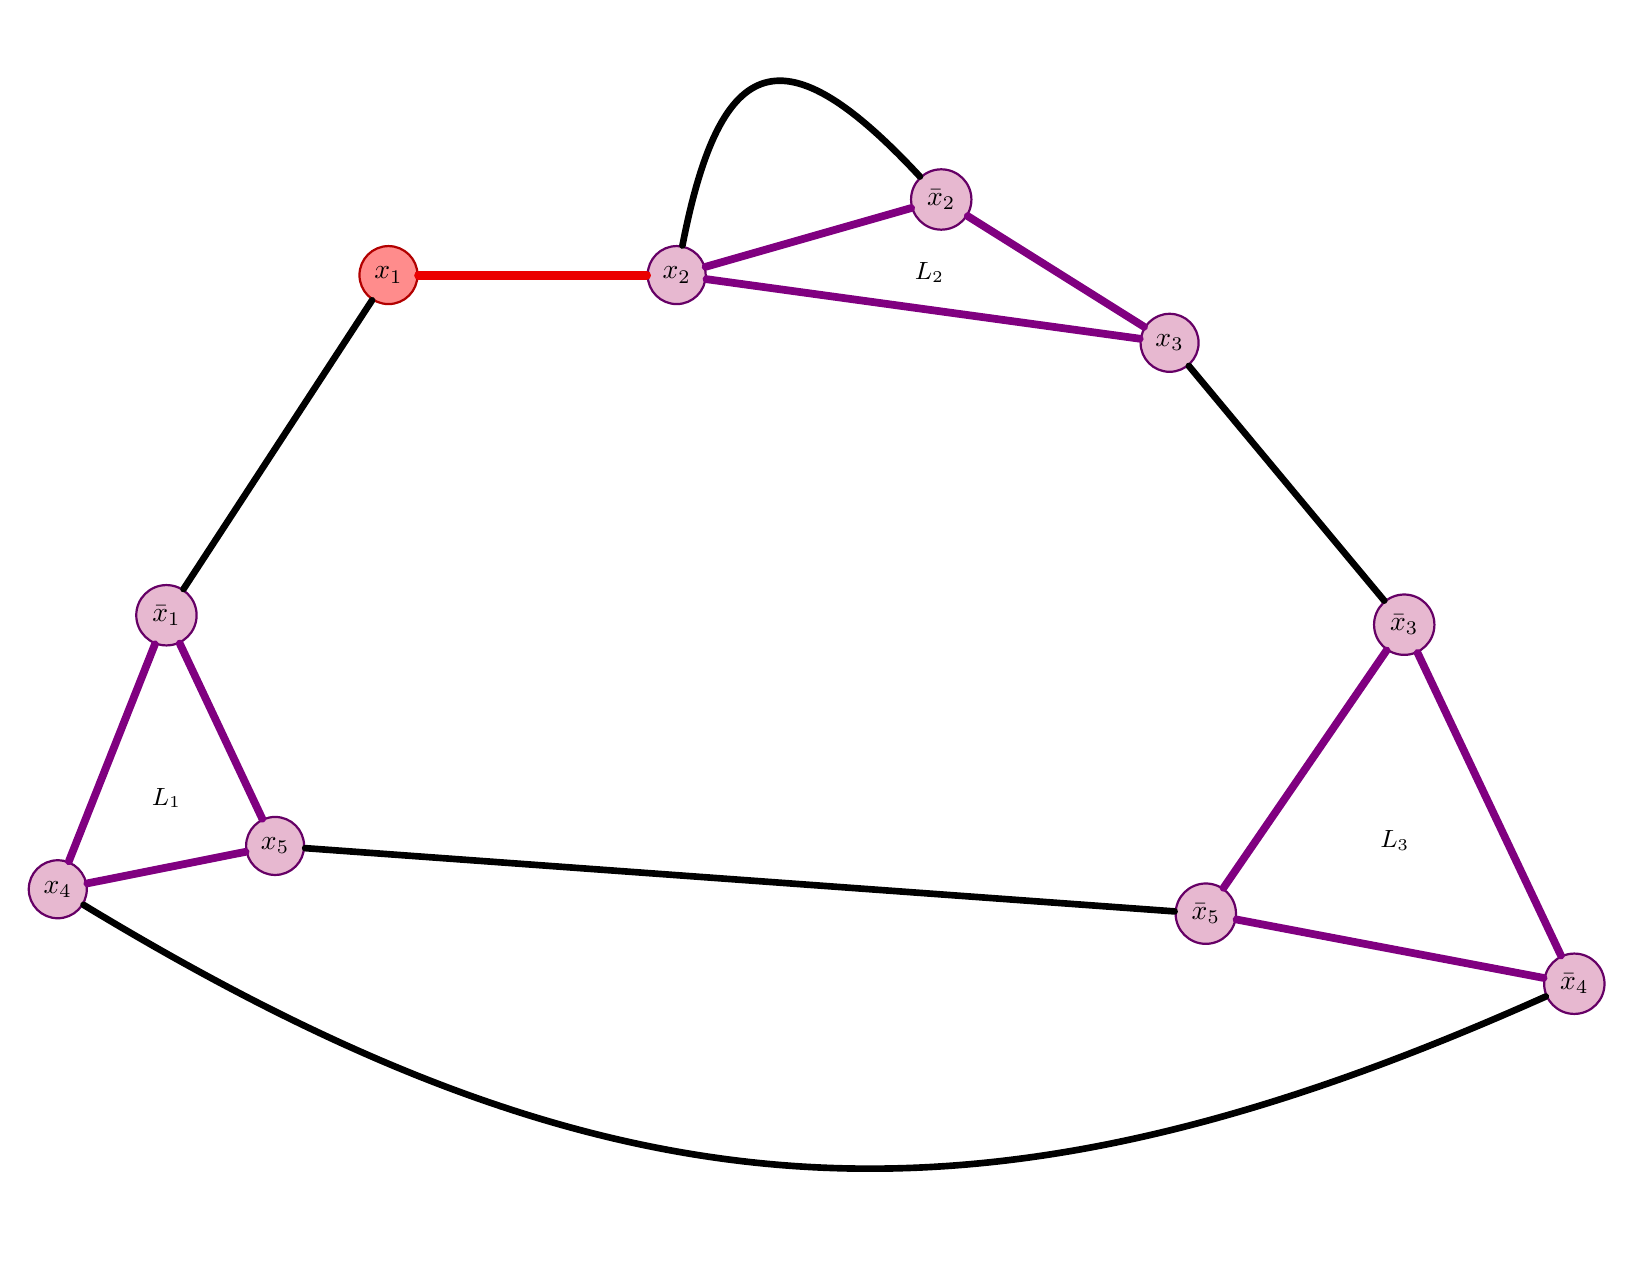
\begin{tikzpicture}[
  lbl/.style={font=\small, inner sep=1pt},
  redv/.style={circle, draw=red!70!black, line width=0.8pt, fill=red!45, minimum size=7mm},
  purpv/.style={circle, draw=violet!80!black, line width=0.8pt, fill=blue!12!purple!28, minimum size=7mm},
  purpleedge/.style={draw=violet, line width=2.8pt, line cap=round, line join=round},
  blackedge/.style={draw=black, line width=2.4pt, line cap=round},
  rededge/.style={draw=red!92!black, line width=3.2pt, line cap=round}
]

\node[redv] (nx1) at (-3.84, 6.18) {$x_{1}$};
\node[purpv] (nb1) at (-6.66, 1.86) {$\bar{x}_{1}$};
\node[purpv] (nx2) at (-0.18, 6.18) {$x_{2}$};
\node[purpv] (nb2) at (3.18, 7.14) {$\bar{x}_{2}$};
\node[purpv] (nx3) at (6.08, 5.32) {$x_{3}$};
\node[purpv] (nb3) at (9.06, 1.74) {$\bar{x}_{3}$};
\node[purpv] (nx4) at (-8.04, -1.62) {$x_{4}$};
\node[purpv] (nb4) at (11.22, -2.82) {$\bar{x}_{4}$};
\node[purpv] (nx5) at (-5.28, -1.07) {$x_{5}$};
\node[purpv] (nb5) at (6.54, -1.93) {$\bar{x}_{5}$};
\draw[purpleedge] (nb1) -- (nx4);
\draw[purpleedge] (nb1) -- (nx5);
\draw[purpleedge] (nx4) -- (nx5);
\draw[purpleedge] (nx2) -- (nb2);
\draw[purpleedge] (nx2) -- (nx3);
\draw[purpleedge] (nb2) -- (nx3);
\draw[purpleedge] (nb3) -- (nb4);
\draw[purpleedge] (nb3) -- (nb5);
\draw[purpleedge] (nb4) -- (nb5);
\draw[blackedge] (nx1) -- (nb1);
\draw[blackedge] (nx2) .. controls (0.38,9.05) and (1.19,9.28) .. (nb2);
\draw[blackedge] (nx3) -- (nb3);
\draw[blackedge] (nx4) .. controls (-0.96,-5.91) and (3.66,-6.20) .. (nb4);
\draw[blackedge] (nx5) -- (nb5);
\draw[rededge] (nx1) -- (nx2);
\node[lbl] at (-6.66, -0.46) {$L_1$};
\node[lbl] at (3.03, 6.21) {$L_2$};
\node[lbl] at (8.94, -1.00) {$L_3$};

\end{tikzpicture}%
}%

\end{center}
\medskip
\subsection*{Class 10 (IX)}
\noindent Representative of this ep-isomorphism class.\\
\noindent Distinguished indices:\\ $\{33, 34, 35, 40, 92, 94, 96, 99, 142, 143, 147, 148, 212, 215, 218, 219, 222, 226, 227, 230, 233, 234, 235, 240\}$, $24$ total.
\begin{center}
\resizebox{\linewidth}{!}{%
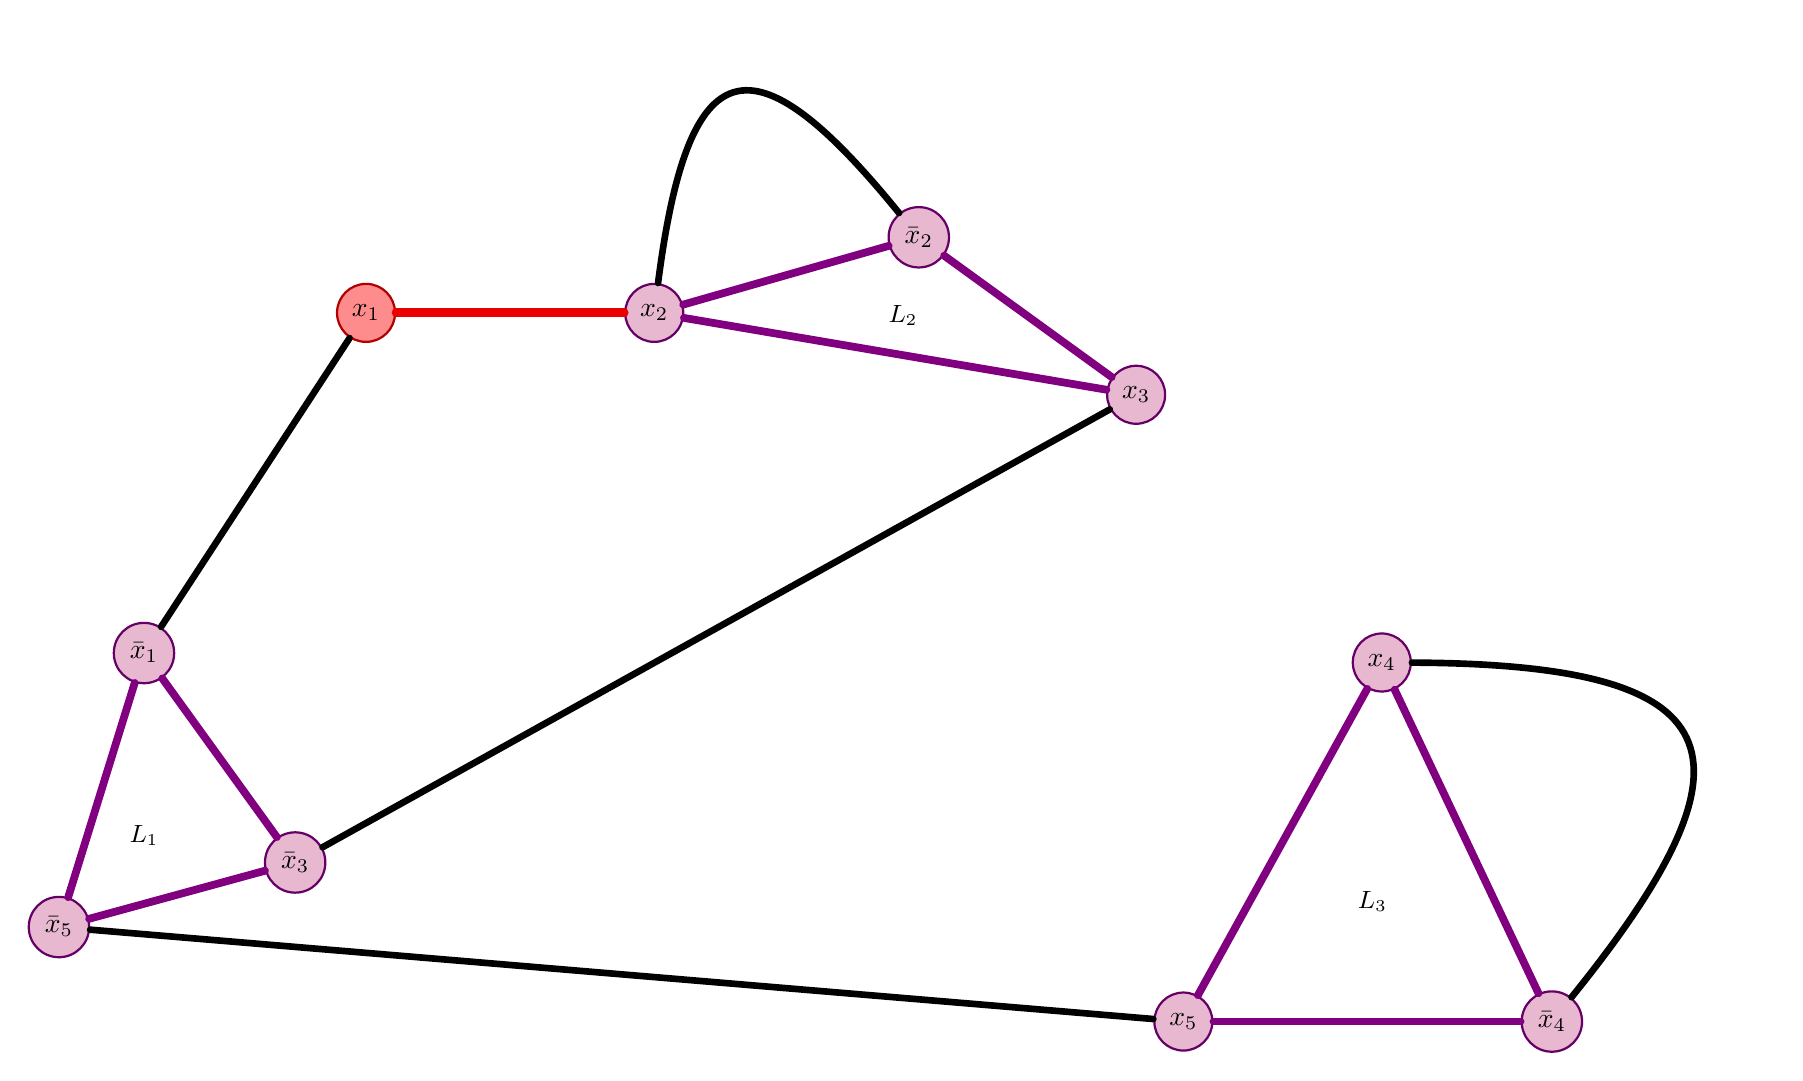
\begin{tikzpicture}[
  lbl/.style={font=\small, inner sep=1pt},
  redv/.style={circle, draw=red!70!black, line width=0.8pt, fill=red!45, minimum size=7mm},
  purpv/.style={circle, draw=violet!80!black, line width=0.8pt, fill=blue!12!purple!28, minimum size=7mm},
  purpleedge/.style={draw=violet, line width=2.8pt, line cap=round, line join=round},
  blackedge/.style={draw=black, line width=2.4pt, line cap=round},
  rededge/.style={draw=red!92!black, line width=3.2pt, line cap=round}
]

\node[redv] (nx1) at (-3.84, 6.18) {$x_{1}$};
\node[purpv] (nb1) at (-6.66, 1.86) {$\bar{x}_{1}$};
\node[purpv] (nx2) at (-0.18, 6.18) {$x_{2}$};
\node[purpv] (nb2) at (3.18, 7.14) {$\bar{x}_{2}$};
\node[purpv] (nx3) at (5.94, 5.14) {$x_{3}$};
\node[purpv] (nb3) at (-4.74, -0.80) {$\bar{x}_{3}$};
\node[purpv] (nx4) at (9.06, 1.74) {$x_{4}$};
\node[purpv] (nb4) at (11.22, -2.82) {$\bar{x}_{4}$};
\node[purpv] (nx5) at (6.54, -2.82) {$x_{5}$};
\node[purpv] (nb5) at (-7.74, -1.62) {$\bar{x}_{5}$};
\draw[purpleedge] (nb1) -- (nb3);
\draw[purpleedge] (nb1) -- (nb5);
\draw[purpleedge] (nb3) -- (nb5);
\draw[purpleedge] (nx2) -- (nb2);
\draw[purpleedge] (nx2) -- (nx3);
\draw[purpleedge] (nb2) -- (nx3);
\draw[purpleedge] (nx4) -- (nb4);
\draw[purpleedge] (nx4) -- (nx5);
\draw[purpleedge] (nb4) -- (nx5);
\draw[blackedge] (nx1) -- (nb1);
\draw[blackedge] (nx2) .. controls (0.25,9.53) and (1.05,9.76) .. (nb2);
\draw[blackedge] (nx3) -- (nb3);
\draw[blackedge] (nx4) .. controls (13.50,1.72) and (14.01,0.63) .. (nb4);
\draw[blackedge] (nx5) -- (nb5);
\draw[rededge] (nx1) -- (nx2);
\node[lbl] at (-6.66, -0.46) {$L_1$};
\node[lbl] at (2.98, 6.15) {$L_2$};
\node[lbl] at (8.94, -1.30) {$L_3$};

\end{tikzpicture}%
}%

\end{center}
\medskip
\subsection*{Class 11 (XIII)}
\noindent Representative of this ep-isomorphism class.\\
\noindent Distinguished indices: $\{36, 38, 95, 98, 145, 149, 213, 217, 223, 228, 236, 238\}$, $12$ total.
\begin{center}
\resizebox{\linewidth}{!}{%
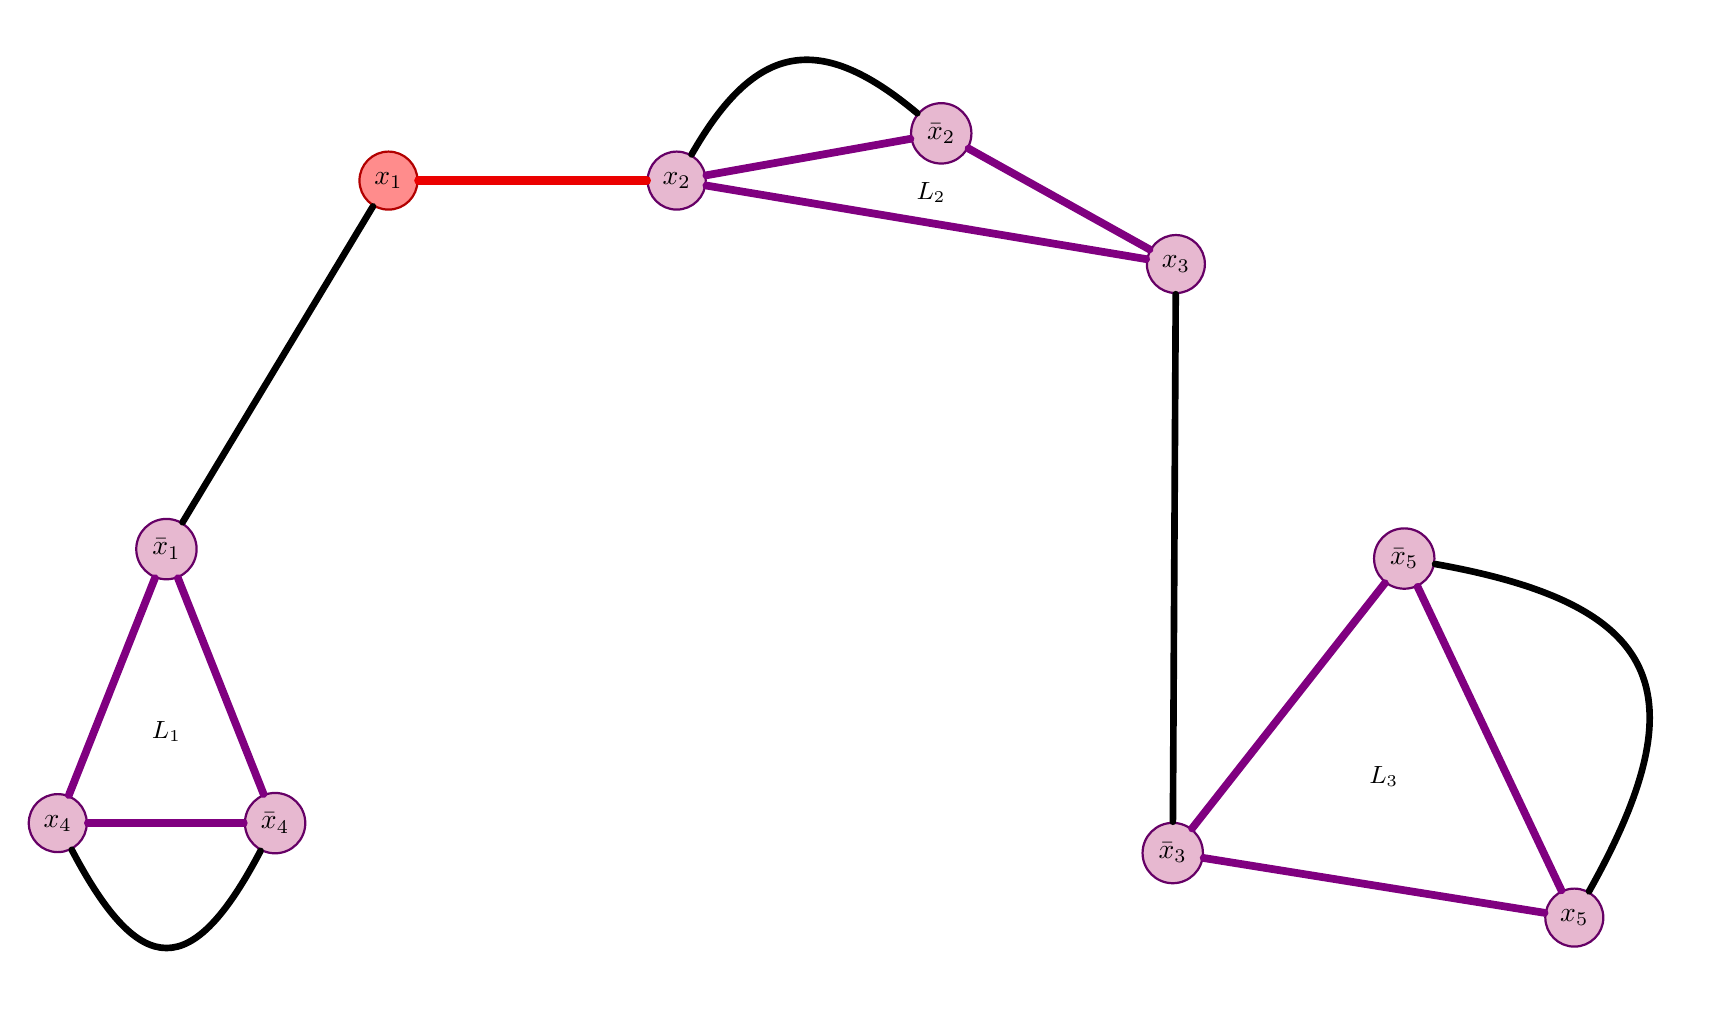
\begin{tikzpicture}[
  lbl/.style={font=\small, inner sep=1pt},
  redv/.style={circle, draw=red!70!black, line width=0.8pt, fill=red!45, minimum size=7mm},
  purpv/.style={circle, draw=violet!80!black, line width=0.8pt, fill=blue!12!purple!28, minimum size=7mm},
  purpleedge/.style={draw=violet, line width=2.8pt, line cap=round, line join=round},
  blackedge/.style={draw=black, line width=2.4pt, line cap=round},
  rededge/.style={draw=red!92!black, line width=3.2pt, line cap=round}
]

\node[redv] (nx1) at (-3.84, 6.54) {$x_{1}$};
\node[purpv] (nb1) at (-6.66, 1.86) {$\bar{x}_{1}$};
\node[purpv] (nx2) at (-0.18, 6.54) {$x_{2}$};
\node[purpv] (nb2) at (3.18, 7.14) {$\bar{x}_{2}$};
\node[purpv] (nx3) at (6.16, 5.48) {$x_{3}$};
\node[purpv] (nb3) at (6.12, -2.00) {$\bar{x}_{3}$};
\node[purpv] (nx4) at (-8.04, -1.62) {$x_{4}$};
\node[purpv] (nb4) at (-5.28, -1.62) {$\bar{x}_{4}$};
\node[purpv] (nx5) at (11.22, -2.82) {$x_{5}$};
\node[purpv] (nb5) at (9.06, 1.74) {$\bar{x}_{5}$};
\draw[purpleedge] (nb1) -- (nx4);
\draw[purpleedge] (nb1) -- (nb4);
\draw[purpleedge] (nx4) -- (nb4);
\draw[purpleedge] (nx2) -- (nb2);
\draw[purpleedge] (nx2) -- (nx3);
\draw[purpleedge] (nb2) -- (nx3);
\draw[purpleedge] (nb3) -- (nx5);
\draw[purpleedge] (nb3) -- (nb5);
\draw[purpleedge] (nx5) -- (nb5);
\draw[blackedge] (nx1) -- (nb1);
\draw[blackedge] (nx2) .. controls (0.82,8.29) and (1.63,8.44) .. (nb2);
\draw[blackedge] (nx3) -- (nb3);
\draw[blackedge] (nx4) .. controls (-6.99,-3.62) and (-6.33,-3.62) .. (nb4);
\draw[blackedge] (nx5) .. controls (12.84,0.07) and (12.32,1.16) .. (nb5);
\draw[rededge] (nx1) -- (nx2);
\node[lbl] at (-6.66, -0.46) {$L_1$};
\node[lbl] at (3.05, 6.39) {$L_2$};
\node[lbl] at (8.80, -1.03) {$L_3$};

\end{tikzpicture}%
}%

\end{center}
\medskip
\subsection*{Class 12 (V)}
\noindent Representative of this ep-isomorphism class.\\
\noindent Distinguished indices: $\{41, 42, 47, 49, 111, 112, 117, 119, 171, 172, 177, 179\}$, $12$ total.
\begin{center}
\resizebox{\linewidth}{!}{%
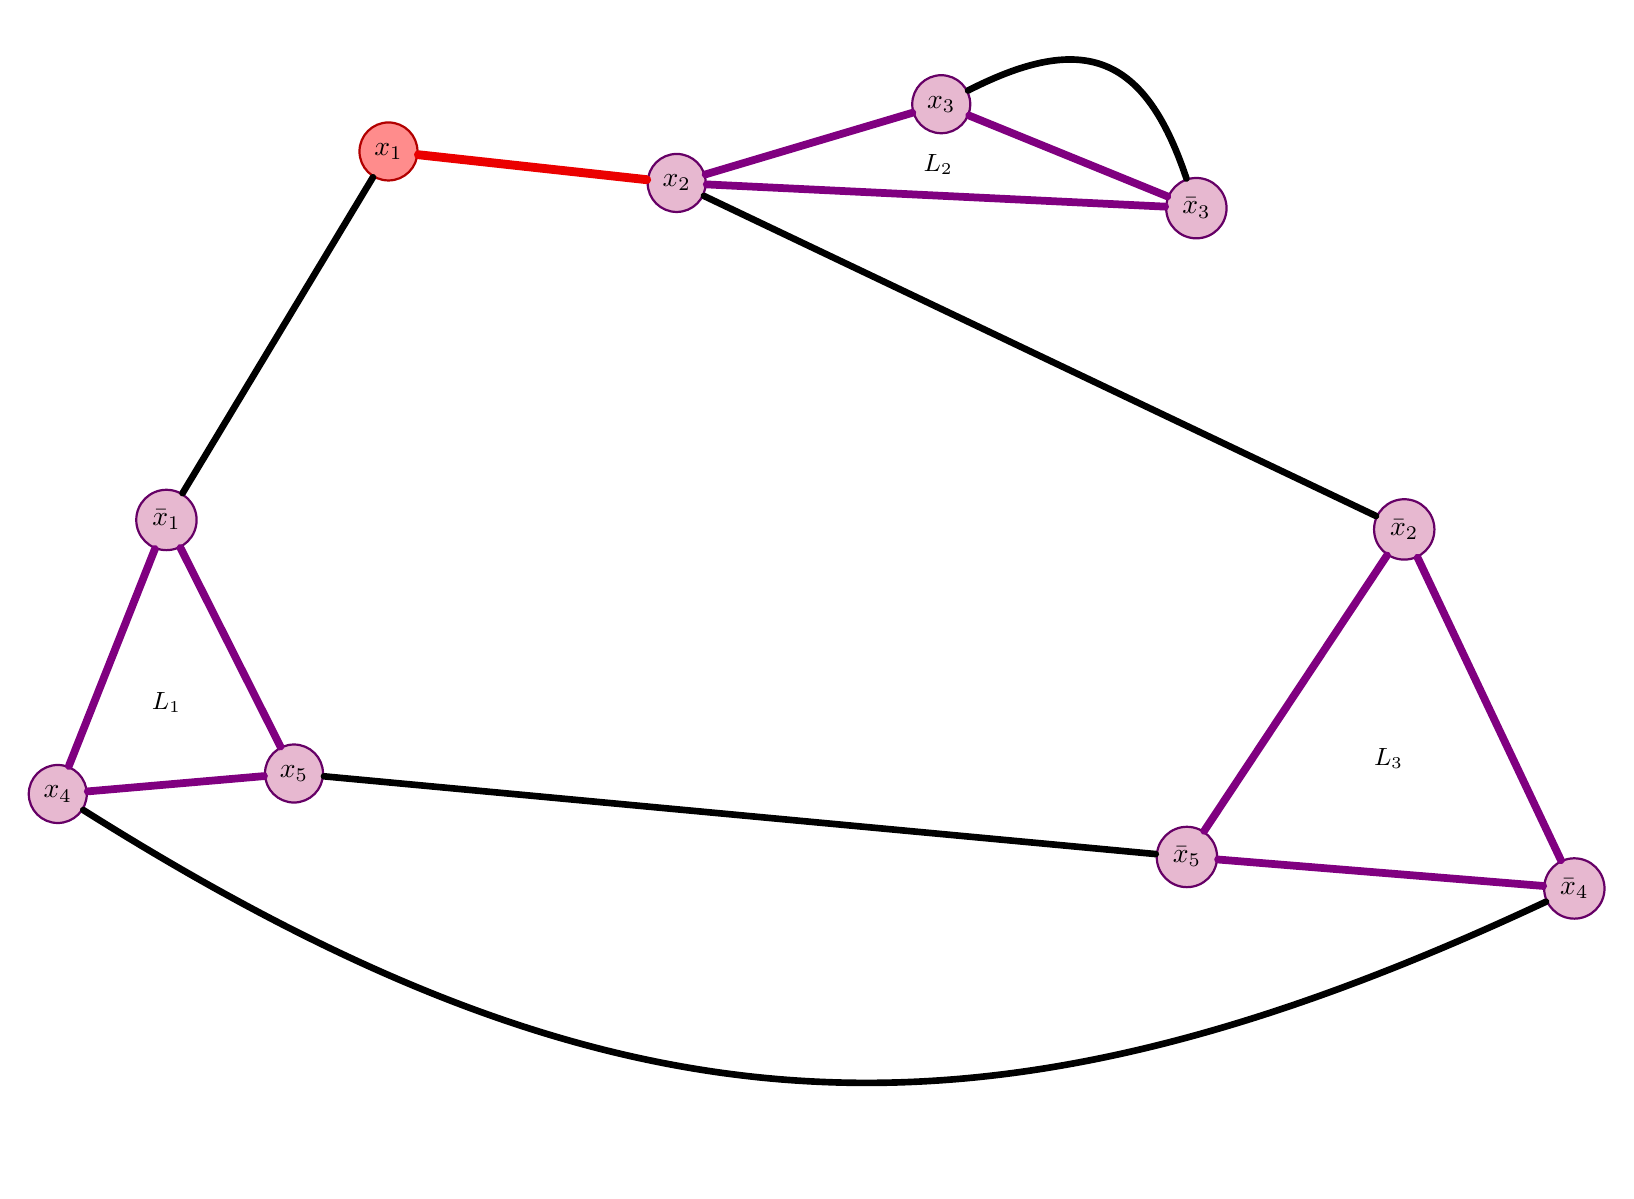
\begin{tikzpicture}[
  lbl/.style={font=\small, inner sep=1pt},
  redv/.style={circle, draw=red!70!black, line width=0.8pt, fill=red!45, minimum size=7mm},
  purpv/.style={circle, draw=violet!80!black, line width=0.8pt, fill=blue!12!purple!28, minimum size=7mm},
  purpleedge/.style={draw=violet, line width=2.8pt, line cap=round, line join=round},
  blackedge/.style={draw=black, line width=2.4pt, line cap=round},
  rededge/.style={draw=red!92!black, line width=3.2pt, line cap=round}
]

\node[redv] (nx1) at (-3.84, 6.54) {$x_{1}$};
\node[purpv] (nb1) at (-6.66, 1.86) {$\bar{x}_{1}$};
\node[purpv] (nx2) at (-0.18, 6.14) {$x_{2}$};
\node[purpv] (nb2) at (9.06, 1.74) {$\bar{x}_{2}$};
\node[purpv] (nx3) at (3.18, 7.14) {$x_{3}$};
\node[purpv] (nb3) at (6.42, 5.82) {$\bar{x}_{3}$};
\node[purpv] (nx4) at (-8.04, -1.62) {$x_{4}$};
\node[purpv] (nb4) at (11.22, -2.82) {$\bar{x}_{4}$};
\node[purpv] (nx5) at (-5.04, -1.36) {$x_{5}$};
\node[purpv] (nb5) at (6.30, -2.42) {$\bar{x}_{5}$};
\draw[purpleedge] (nb1) -- (nx4);
\draw[purpleedge] (nb1) -- (nx5);
\draw[purpleedge] (nx4) -- (nx5);
\draw[purpleedge] (nx2) -- (nx3);
\draw[purpleedge] (nx2) -- (nb3);
\draw[purpleedge] (nx3) -- (nb3);
\draw[purpleedge] (nb2) -- (nb4);
\draw[purpleedge] (nb2) -- (nb5);
\draw[purpleedge] (nb4) -- (nb5);
\draw[blackedge] (nx1) -- (nb1);
\draw[blackedge] (nx2) -- (nb2);
\draw[blackedge] (nx3) .. controls (5.00,8.07) and (5.77,7.76) .. (nb3);
\draw[blackedge] (nx4) .. controls (-0.97,-6.07) and (3.65,-6.36) .. (nb4);
\draw[blackedge] (nx5) -- (nb5);
\draw[rededge] (nx1) -- (nx2);
\node[lbl] at (-6.66, -0.46) {$L_1$};
\node[lbl] at (3.14, 6.37) {$L_2$};
\node[lbl] at (8.86, -1.17) {$L_3$};

\end{tikzpicture}%
}%

\end{center}
\medskip
\subsection*{Class 13 (XI)}
\noindent Representative of this ep-isomorphism class.\\
\noindent Distinguished indices: $\{43, 44, 45, 50, 113, 114, 115, 120, 173, 174, 175, 180\}$, $12$ total.
\begin{center}
\resizebox{\linewidth}{!}{%
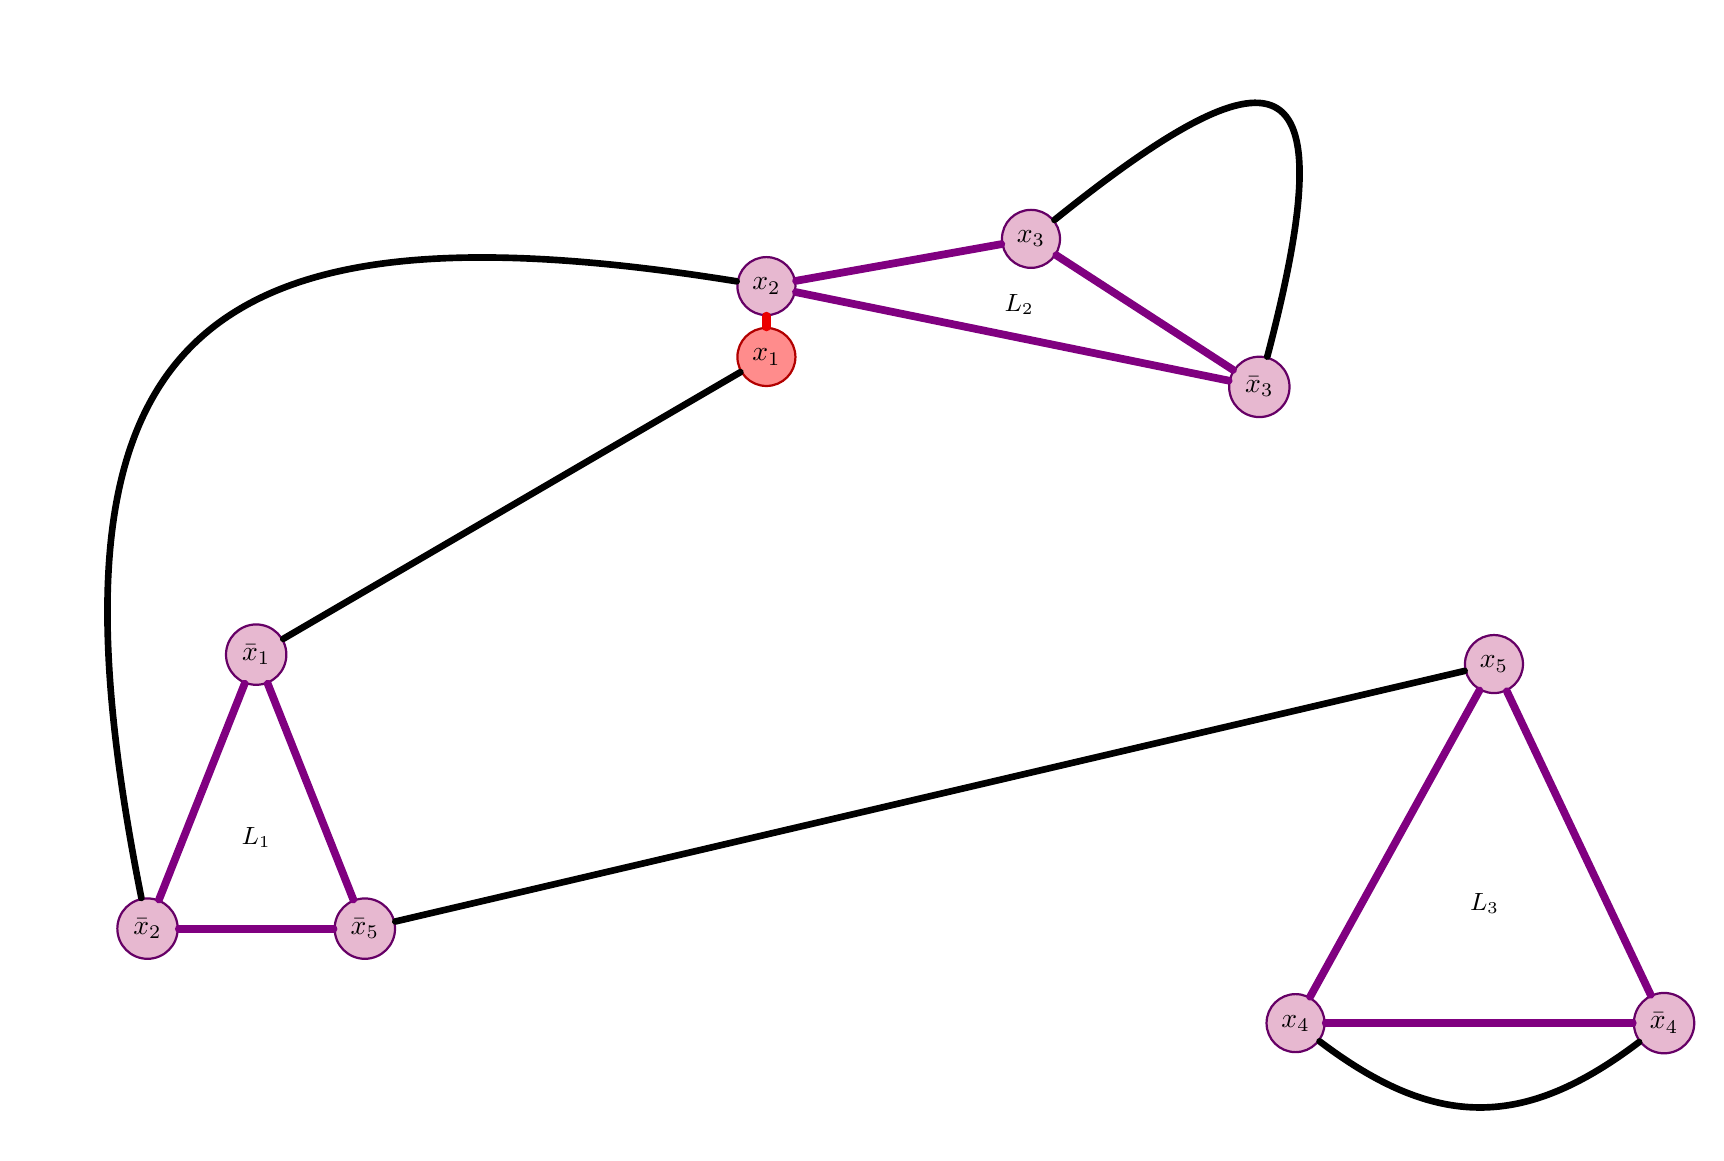
\begin{tikzpicture}[
  lbl/.style={font=\small, inner sep=1pt},
  redv/.style={circle, draw=red!70!black, line width=0.8pt, fill=red!45, minimum size=7mm},
  purpv/.style={circle, draw=violet!80!black, line width=0.8pt, fill=blue!12!purple!28, minimum size=7mm},
  purpleedge/.style={draw=violet, line width=2.8pt, line cap=round, line join=round},
  blackedge/.style={draw=black, line width=2.4pt, line cap=round},
  rededge/.style={draw=red!92!black, line width=3.2pt, line cap=round}
]

\node[redv] (nx1) at (-0.18, 5.64) {$x_{1}$};
\node[purpv] (nb1) at (-6.66, 1.86) {$\bar{x}_{1}$};
\node[purpv] (nx2) at (-0.18, 6.54) {$x_{2}$};
\node[purpv] (nb2) at (-8.04, -1.62) {$\bar{x}_{2}$};
\node[purpv] (nx3) at (3.18, 7.14) {$x_{3}$};
\node[purpv] (nb3) at (6.08, 5.26) {$\bar{x}_{3}$};
\node[purpv] (nx4) at (6.54, -2.82) {$x_{4}$};
\node[purpv] (nb4) at (11.22, -2.82) {$\bar{x}_{4}$};
\node[purpv] (nx5) at (9.06, 1.74) {$x_{5}$};
\node[purpv] (nb5) at (-5.28, -1.62) {$\bar{x}_{5}$};
\draw[purpleedge] (nb1) -- (nb2);
\draw[purpleedge] (nb1) -- (nb5);
\draw[purpleedge] (nb2) -- (nb5);
\draw[purpleedge] (nx2) -- (nx3);
\draw[purpleedge] (nx2) -- (nb3);
\draw[purpleedge] (nx3) -- (nb3);
\draw[purpleedge] (nx4) -- (nb4);
\draw[purpleedge] (nx4) -- (nx5);
\draw[purpleedge] (nb4) -- (nx5);
\draw[blackedge] (nx1) -- (nb1);
\draw[blackedge] (nx2) .. controls (-7.63,7.74) and (-9.52,5.78) .. (nb2);
\draw[blackedge] (nx3) .. controls (6.46,9.78) and (7.15,9.33) .. (nb3);
\draw[blackedge] (nx4) .. controls (8.32,-4.17) and (9.44,-4.17) .. (nb4);
\draw[blackedge] (nx5) -- (nb5);
\draw[rededge] (nx1) -- (nx2);
\node[lbl] at (-6.66, -0.46) {$L_1$};
\node[lbl] at (3.03, 6.31) {$L_2$};
\node[lbl] at (8.94, -1.30) {$L_3$};

\end{tikzpicture}%
}%

\end{center}
\medskip
\subsection*{Class 14 (XIV)}
\noindent Representative of this ep-isomorphism class.\\
\noindent Distinguished indices: $\{46, 48, 116, 118, 176, 178\}$, $6$ total.
\begin{center}
\resizebox{\linewidth}{!}{%
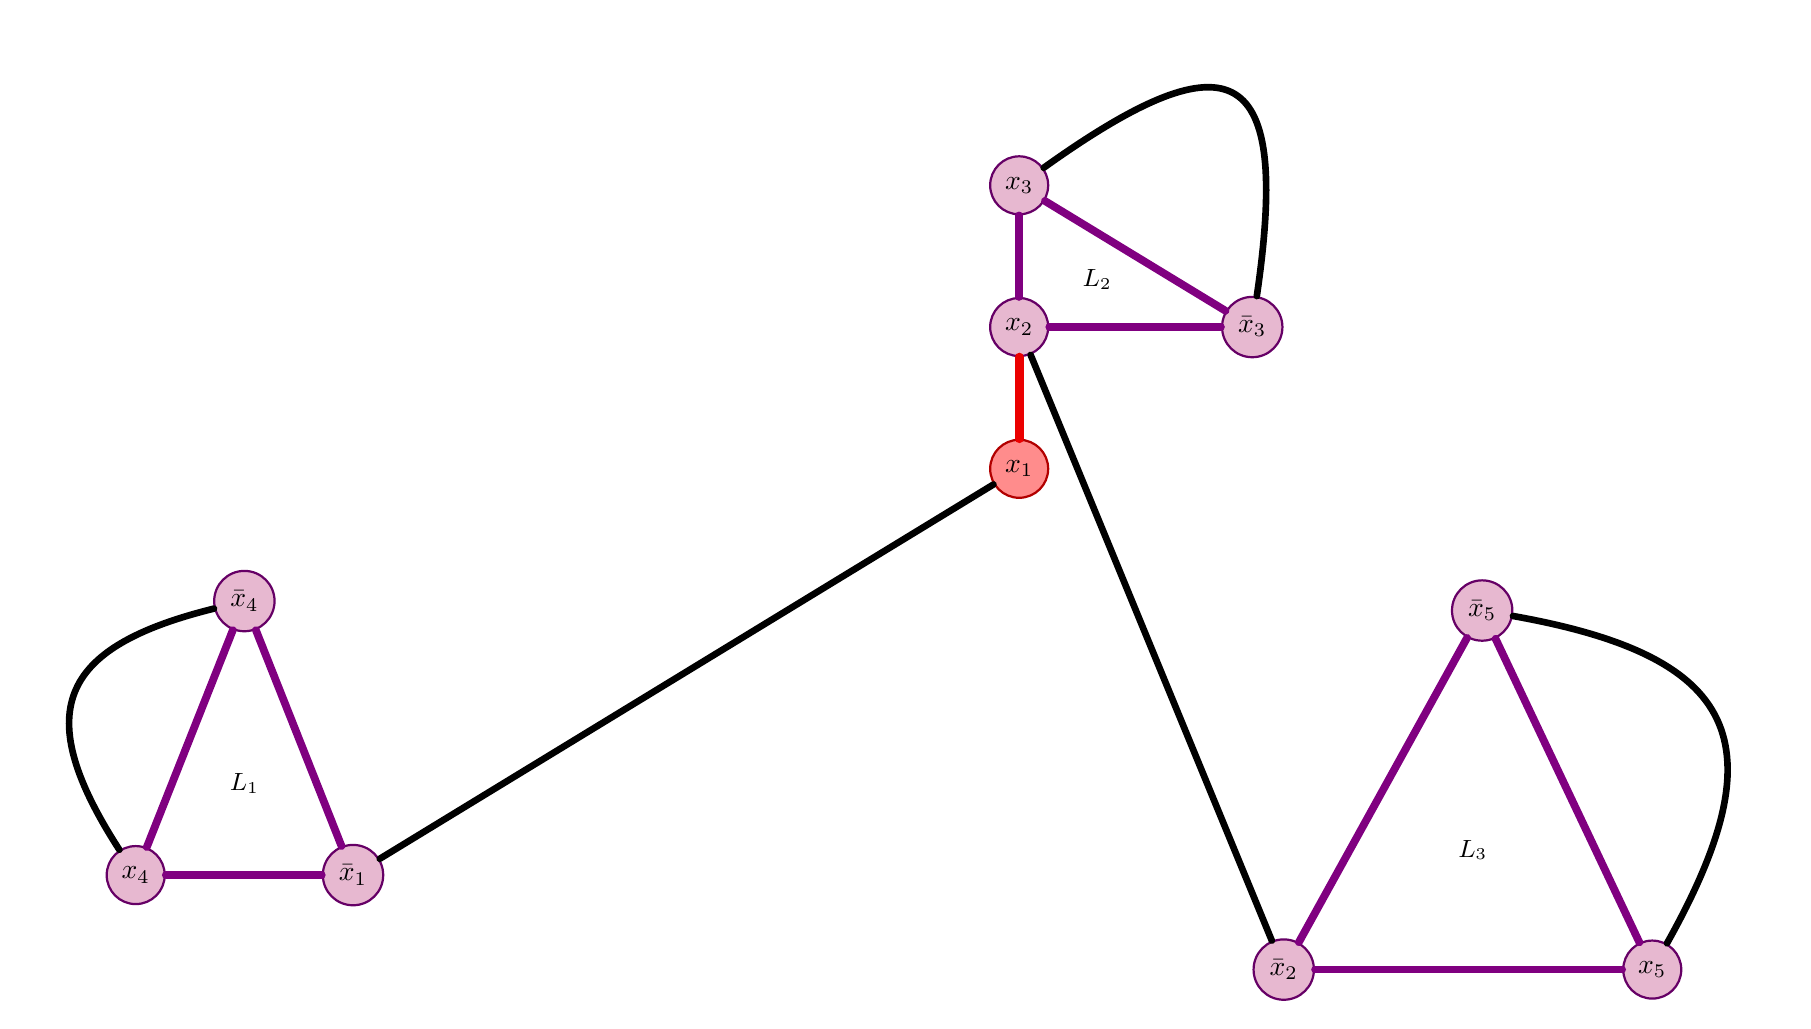
\begin{tikzpicture}[
  lbl/.style={font=\small, inner sep=1pt},
  redv/.style={circle, draw=red!70!black, line width=0.8pt, fill=red!45, minimum size=7mm},
  purpv/.style={circle, draw=violet!80!black, line width=0.8pt, fill=blue!12!purple!28, minimum size=7mm},
  purpleedge/.style={draw=violet, line width=2.8pt, line cap=round, line join=round},
  blackedge/.style={draw=black, line width=2.4pt, line cap=round},
  rededge/.style={draw=red!92!black, line width=3.2pt, line cap=round}
]

\node[redv] (nx1) at (3.18, 3.54) {$x_{1}$};
\node[purpv] (nb1) at (-5.28, -1.62) {$\bar{x}_{1}$};
\node[purpv] (nx2) at (3.18, 5.34) {$x_{2}$};
\node[purpv] (nb2) at (6.54, -2.82) {$\bar{x}_{2}$};
\node[purpv] (nx3) at (3.18, 7.14) {$x_{3}$};
\node[purpv] (nb3) at (6.14, 5.34) {$\bar{x}_{3}$};
\node[purpv] (nx4) at (-8.04, -1.62) {$x_{4}$};
\node[purpv] (nb4) at (-6.66, 1.86) {$\bar{x}_{4}$};
\node[purpv] (nx5) at (11.22, -2.82) {$x_{5}$};
\node[purpv] (nb5) at (9.06, 1.74) {$\bar{x}_{5}$};
\draw[purpleedge] (nb1) -- (nx4);
\draw[purpleedge] (nb1) -- (nb4);
\draw[purpleedge] (nx4) -- (nb4);
\draw[purpleedge] (nx2) -- (nx3);
\draw[purpleedge] (nx2) -- (nb3);
\draw[purpleedge] (nx3) -- (nb3);
\draw[purpleedge] (nb2) -- (nx5);
\draw[purpleedge] (nb2) -- (nb5);
\draw[purpleedge] (nx5) -- (nb5);
\draw[blackedge] (nx1) -- (nb1);
\draw[blackedge] (nx2) -- (nb2);
\draw[blackedge] (nx3) .. controls (5.92,9.10) and (6.63,8.67) .. (nb3);
\draw[blackedge] (nx4) .. controls (-9.37,0.44) and (-9.04,1.27) .. (nb4);
\draw[blackedge] (nx5) .. controls (12.84,0.07) and (12.32,1.16) .. (nb5);
\draw[rededge] (nx1) -- (nx2);
\node[lbl] at (-6.66, -0.46) {$L_1$};
\node[lbl] at (4.17, 5.94) {$L_2$};
\node[lbl] at (8.94, -1.30) {$L_3$};

\end{tikzpicture}%
}%

\end{center}
\medskip